\begin{displayquote}
	\textsf{In Chapter \ref{Krylov Subspace Methods}, we have discussed the convergence of iterative methods and its relation with spectral distribution of linear systems. Indeed, algorithms and applications from diverse fields can be formulated as eigenvalue problems. The eigenvalues are also extremely important for the preconditioners of solving linear systems. In machine learning and pattern recognition, it is often demanded to solve the eigenvalue problems for both supervised and unsupervised learning algorithms, such as PCA \cite{croux2000principal}, FDA \cite{berkes2005handwritten}, and clustering \cite{fender2017parallel}, etc. An insufficient accuracy and a failure of eigenvalue solvers and linear solvers usually result in, respectively, a poor approximation to original discrete problems and failure of entire algorithms.  A good selection of solvers becomes especially essential. Thus it is crucial to have the test matrices to benchmark the numerical performance and parallel efficiency of different methods. In this chaper, we present SMG2S, including its parallel implementation and optimization of both CPU and GPU clusters, the verification mechanism, and the release of the open source package.}
\end{displayquote}

\vspace{0.6in}

\section{Demand of Large Matrices with Given Spectrum}

As presented in Chapter \ref{Krylov Subspace Methods}, nowadays, the size of eigenvalue problems and the supercomputer systems continue to scale up. The whole ecosystem of HPC, especially the linear system applications, should be adjusted to this kind of large clusters. Under this background, there are four special requirements on the test matrices for the evaluation of numerical algorithms on extreme-scale platforms: 

\begin{enumerate}[label=(\arabic*)]
	\item their spectra must be known and can be customized;
	\item they should be both sparse, non-Hermitian and non-trivial;
	\item they could have a very high dimension, including the non-zero element numbers and/or the matrix dimension, to evaluate the numerical algorithms on large-scale systems, which means that the proposed matrix generator should be able to be parallelized to profit from the large distributed memory clusters.
	\item their sparsity patterns should be controllable.
\end{enumerate}

In order to provide numerically robust solvers of eigenvalue or linear system problems, the researchers need the matrices whose spectra are known, which help to analyze the numerical accuracy. Some scientific communities may be interested in matrices with clustered, conjugated eigenvalues, the closest eigenvalues in random distribution or contained in a specified interval. It is significant to develop a suite of large non-Hermitian test matrices whose eigenvalues can be given.

The properties of being sparse, non-Hermitian and non-trivial together can add many mathematical features to simulate the matrices in reality. Besides, the test matrices should have very high dimensions for the experiments on large-scale platforms. Furthermore, since the large matrix is generated in a parallel way, its different slices are already distributed on separate computing units, which can be directly used to evaluate the required linear and eigenvalue solvers, without concerning loading the large matrix file from the filesystems. It can save time and improve the efficiency for the applications.

In this chapter, we present SMG2S for testing the linear and eigenvalue solvers on large-scale platforms. In Section \ref{Existing Collections}, we introduce the related work to propose test matrix collections. In Section \ref{Mathematical Framework}, we give the proof of mathematical framework of SMG2S to generate matrices with given spectra. In Section \ref{Matrix_Generation_Method}, the numerical algorithm and practical implementation of SMG2S are presented. In section \ref{Parallel Impementation and Evaluation}, firstly, we provide a naive implementation of SMG2S based on PETSc\footnote{Portable, Extensible Toolkit for Scientific Computation.} for homogenous platforms and PETSc+CUDA\footnote{Compute Unified Device Architecture} for heterogeneous machines with multi-GPU. Then an open source package\footnote{https://github.com/smg2s/SMG2S} with specific communication optimization based on MPI\footnote{Message Passing Interface.} and C++ is available.  In Section \ref{Parallel Performance Evaluation}, the evaluations of its scalability and the accuracy to keep the given spectra are presented on different supercomputing platforms.  A mechanism to verify the capacity of the generated matrix to keep the given spectra has been proposed based on the Shifted Inverse Power Method in Section \ref{Verification Method}, and the accuracy verification for various spectral distribution is also presented in this section. In Section \ref{Package, Interface and Application}, we introduce the SMG2S package as a released software, including the interfaces to different programming languages and scientific computational libraries, the GUI for verification. Finally an example using SMG2S to evaluate the Krylov solvers is given in Section \ref{application}. 

\section{The Existing Collections} \label{Existing Collections}

It's rare, but there are already several efforts to supply test matrix collections for linear problems. SPARSEKIT \cite{saad1994sparsekit} implemented by Y. Saad contains various simple matrix generation subroutines. Z. Bai et al. \cite{bai1996test} presented a collection of test matrices for the development of numerical algorithms for solving nonsymmetric eigenvalue problems. There are also two widely spread matrix providers, the Tim Davis collection \cite{davis2011university} and Matrix Market \cite{boisvert1997matrix}. They all contain many matrices with various mathematical properties coming from different scientific fields. However, the spectra of matrices in these collections are fixed, and that cannot be whatever we want. A test matrix generation suite with given spectra was already introduced by J. Demmel et al. \cite{demmel1989test} in 1989 for the benchmark of LAPACK\footnote{Linear Algebra PACKage}. They proposed the method to transfer the diagonal matrix with given spectra into a dense matrix with same spectra using the orthogonal matrices, and then reduce them to unsymmetric band ones by the Householder transformation. This method requires $\mathcal{O}(n^3)$ time and $\mathcal{O}(n^2)$ storage even for generating a small bandwidth matrix. Moreover, this method was implemented for the shared memory systems, not for larger distributed memory systems. Thus it is difficult to generate large-scale test matrices customized for the tests on extreme scale clusters. That is the motivation for us to propose SMG2S which can generate large-scale non-Hermitian matrices with given spectra on modern parallel platforms with much less time and storage, and easily be implemented in distributed memory systems.

\iffalse
\subsection{Matrix Generators In LAPACK}

In LAPCK, a suite of test matrix generation software is implementation, which generates random matrices with various controlled properties. The three mains routines are called xLATMR, xLATMS and xLATME, where the first letter of each name is either 'S', 'D', 'C', or 'Z'. They signficate respectively the entries to be 'single-precision real', 'double-precision real', 'single-precision complex' and 'double-precision complex'.

\subsubsection{xLATMR, xLATMS and xLATME}

xLATMR generates a random matrix with off-diagonal entries,  It is the simplest and fastest routines in this suite, and permits no direct control over the eigenvalues of the generated matrices, the properties of xLATMR is given as:

\begin{itemize}
	\item Elements of $A$ formed from one of three distributions
	\item Symmetric or nonsymmetric.
	\item Optionally graded (by row and/or column), banded, "sparsified".
	\item Bandwidth optionally reduced to a specified value.
\end{itemize}

xLATMS generates random real symmetric and complex Hermitian matrices with given eigenvalues and bandwidth, or a random nonsymmetric or complex symmetric matrix with given singular values and upper and lower bandwidth.

\begin{itemize}
	\item Matrix of singular values specified by the user or chosen from one of six different distributions.
	\item $A$ is formed as $UDV^T$, where $V$ is random orthogonal.
	\item Bandwidth optionally reduced to a specified value by further unitary transformations (possibly combined with the previous step).
\end{itemize}

xLATME generates a random nonsymmetric square matrix with specified eigenvalues. For example, xLATME is able to generate random Hessenberg matrices with given eigenvalues and sensitivities, and this is useful for testing QR factorization algorithms for nonsymmetric eigenproblems. In the practical implementation, only dense matrix storage format is supported, hence, xLATME uses $n^2+\mathcal{O}(n)$ space and $\mathcal{O}(n^3)$ time. The procedure of generation matrix by xLATME can be given as follows:

\begin{enumerate}
	\item User can specify the diagonal of $A$ by $D=diag(\lambda_i)$, and the entries of $D$ can be computed as follows:
	\begin{enumerate}
		\item Input by users;
		\item $D(1)=1$ and the other $D(i)=\frac{1}{COND}$, where $COND$ is the condition number specified by the users;
		\item $D(n)=\frac{1}{COND}$ and the other $D(i)=1$;
		\item The $D(i)$ form a geometric sequence from $1$ to $\frac{1}{COND}$;
		\item The $D(i)$ form a arithmetic sequence from $1$ to $\frac{1}{COND}$;
		\item The $D(i)$ are random in the range [$\frac{1}{COND}$, $1$] with uniformly distribuetd logarithms;
		\item The $D(i)$ are random with the same distribution as the othter matrix entries;
	\end{enumerate}
	
	Additionally, each $D(i)$ may optionally be multiplied by a random number with absolute value $1$.
	
	\item If $A$ is real and complex conjugate pairs of eigenvalues are desired, certain pairs of adjacent elements of $D$ are interpreted as the real and imaginary parts of a complex conjugate pair of eigenvalues, and $A$ is made block diagonal with $2 \times 2$ blocks in the corresponding locations. If $D$ is input by the user, the user also specifies which entries are to be interpreted as real and imaginary parts of complex conjugate eigenpairs. If $D$ is not input by the user, the user may specify that pairs of adjacent entries be randomly designated as either a pair of real eigenvalues or as real and imaginary parts of an eigenpair.
	
	\item If the user so specifies, the upper triangle of $A$ is filled with random numbers. This option may be used to control the Jordan form of $A$ as follows partially: if $A$ has any multiple eigenvalues (as determined by the last two steps), and the upper triangle is filled in, then there will be exactly one Jordan block per distinct eigenvalue; such a matrix is called defective. If the upper triangle is not filled in, there will only be $1\times1$ blocks in the Jordan form, even if there are multiple eigenvalues; such a matrix is called derogatory,
	
	\item If the user so specifies, $A$ is premultiplied by a random matrix $S$ and post-multiplied by $S^{-1}$. Here, $S$ is a random dense nonsymmetric matrix whose singular values may be chosen with the same options as $D$. 
	\item If the user so specifies, either the upper or lower bandwidth (but not both) is reduced to any positive value desired.
	\item Scale $A$, if desired, to have a given maximum absolute entry.
\end{enumerate}

\subsubsection{Generating Radom Orthogonal}

The generation of random orthogonal is developed by Stewart \cite{stewart1980efficient}. Let the $x_i \in \mathbb{R}^i$ be independent vectors from the Normal (0,1) distribution. Form 

\begin{equation}
Q=DP_1P_2\cdots P_{n-1}
\end{equation}

where $P_i=diag(I_{n-i},\bar{P}_i)$, where $\bar{P}_i$ is the Householder transformation that reduces $x_i$ to $r_iie_1$ and $D=diag(sign(r_{ii}))$. Then $Q$ is from the Haar distribution.
\fi

\section{SMG2S Mathematical Framework}\label{Mathematical Framework}

In this section, we give a summary of the theorem and related proof based on the preliminary theoretical research of H. Gachlier et al. \cite{galichergenerate}.


\begin{theorem}
	\label{theo1}
	Let's consider the matrices $A \in \mathbb{C}^{n \times n}$, $M_0  \in \mathbb{C}^{n \times n}$, $n \in \mathbb{N}^*$. If M verifies: 
	\[
	\left\{\
	\begin{aligned}
	&\frac{dM(t)}{dt} = AM(t) - M(t)A, \\
	&M(t=0) = M_0. \\ 
	\end{aligned}
	\right.
	\]
	Then the matrices $M(t)$ and $M_0$ are similar, $\forall A \in \mathbb{C}^{n \times n}$. 
\end{theorem}

\begin{proof}
	
	
	Denote respectively $\sigma(M_0)$ and $\sigma(M_t)$ the spectra of $M_0$ and $M_t$. If $M_0$ is a diagonalisable matrix, $\forall \lambda \in \sigma(M_0)$, it exists an eigenvector $v \neq 0$ satisfies the relation:
	\begin{equation}
	M_0 v=\lambda v.
	\end{equation}
	
	Denote $v(t)$ by the matrix $B \in {I}_{n}$:
	
	\begin{equation}
	\label{pf3}
	v(t) = B_tv = e^{tA}Bv.
	\end{equation}
	
	We can get: 
	\begin{equation}
	\begin{aligned}
	\label{proof1}
	\frac{d(M_tv(t) - \lambda v(t))}{dt} &= \frac{dM_t}{dt}v(t) + M_t \frac{dv(t)}{dt} - \lambda \frac{dv(t)}{dt} \\
	&=A(M_t v(t)-\lambda v(t)) + \lambda Av(t) \\&-M_tAv(t)+M_t \frac{dB_t}{dt} v - \lambda \frac{dB_t}{dt} v.
	\end{aligned}
	\end{equation}
	
	With the definition of $B_t$ in Equation (\ref{pf3}), we have:
	
	\begin{equation}
	\frac{dB_t}{dt} = AB_t.
	\end{equation}
	
	Thus the Equation (\ref{proof1}) can be simplified as 
	
	\begin{equation}
	\label{pf4}
	\begin{aligned}
	\frac{d(M_tv(t) - \lambda v(t))}{dt} &=A(M_t v(t) - \lambda v(t)).
	\end{aligned}
	\end{equation}
	
	The initial condition for the Equation (\ref{pf4}) is:
	\begin{equation}
	\begin{aligned}
	M_tv(t) - \lambda v(t)|_{t=0} &= M_0 B v - \lambda B v \\
	& = M_0 v - \lambda v \\
	&= 0.
	\end{aligned}
	\end{equation}
	
	Hence the solution of the differential Equation (\ref{pf4})  is $0$ and $\forall \lambda \in \sigma(M_0)$, we have $\lambda \in \sigma(M_t)$. Since $dim(M_0) = dim(M_t)$, we have $\sigma(M_0) = \sigma(M_t)$. Thus, $M_0$ and $M_t$ are similiar with same eigenvalues, but different eigenvectors.
	
	
\end{proof}

\section{Numerical Implementation of SMG2S} \label{Matrix_Generation_Method}
Base on the previous mathematical work by H. Gachlier, a matrix $M_0$ with given spectra can be transferred to another one $M(t)$ that verifies $Theorem$ $\ref{theo1}$ and keeps the spectra of $M_0$. We propose a matrix generation method by selecting many parameters including the matrices $A$ and $M_0$. 

\subsection{Matrix Generation Method}

The idea is to impose the desired spectra to $M_0$ and obtain a $M_t$ matrix that verifies the Theorem \ref{theo1} and our hypothesis. The $M_t$ spectrum is the same as $M_0$ however we recall that the $M_t$ eigenvectors are not the same as $M_0$. The idea may seem very simple, but many parameters need to be fixed to achieve our objective.

Firstly, we define the linear operator $\widetilde{A}$ such that:

\begin{equation}
\left\{\
\begin{aligned}
A_A: &M_{n \times n} \rightarrow M_{n \times n}, \\
&M \rightarrow  AM-MA. \\ 
\end{aligned}
\right.
\end{equation}

At the present time, we did not imposed any conditions on the matrix $A$. The $\widetilde{A_A}$
operator verifies that:

\begin{equation}
\begin{aligned}
\widetilde{A_A}(I_d)=0, \forall A \in M_{n \times n}. \\ 
\end{aligned}
\end{equation}

Based on the Theorem \ref{theo1} and the linear operator $\widetilde{A_A}$ definition, we can rewritte the
ordinary differential equation such that:

\begin{equation}
\label{eq3}
\left\{\
\begin{aligned} 
&\frac{dM(t)}{dt} =  \widetilde{A_A}(M(t)), \\ 
&M(t=0) =  M_0.
\end{aligned}
\right.
\end{equation}

Starting out the Equation (\ref{eq3}), we apply the exponential operator (which is possible as $\bar{A_A}$ has no time dependency). This leads to the fact that the solution of Equation  (\ref{eq3}), can be expressed as follows:

\begin{equation}
\label{eq4}
\left\{\
\begin{aligned} 
&M_t = e^{(\widetilde{A_At})}M_0, \\ 
&M_t=\sum_{k=0}^{\infty} \frac{t^k}{k!}(\widetilde{A_A})^kM_0.
\end{aligned}
\right.
\end{equation}

The $k$-times power operation of $\widetilde{A_A}(M_0)$ can be given as
\begin{equation}
(\widetilde{A_A})^k(M_0)=\sum_{m=0}^{k}(-1)^mC_k^mA^{k-m}M_0A^m.
\end{equation}

With the loop 
\begin{equation}
M_{i+1}=M_i+\frac{1}{i!}(\widetilde{A_A})^i(M_0), i\in(0,+\infty),
\end{equation}

a very simple initial matrix $M_0 \in \mathbb{C}^{n \times n}$ can be transfered into a new sparse, non-trivial and non-Hermitian matrix $M_{+\infty} \in \mathbb{C}^{n \times n}$, which has the same spectra but different eigenvectors with $M_0$.

\begin{figure}[t]
	\centering
	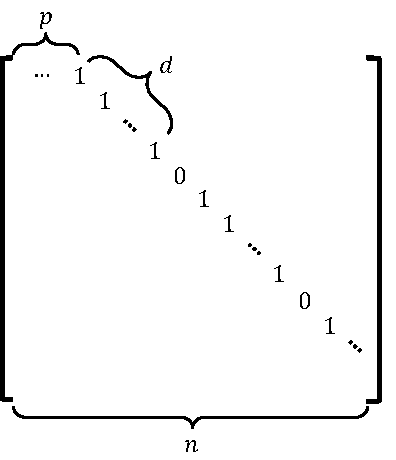
\includegraphics[width=3.0in]{fig/nilpotent_matrix.pdf}
	\caption{Nilpotent Matrix. $p$ off-diagonal offset, $d$ number of continuous $1$, and $n$ matrix dimension.}
	\label{fig:nilpotent}
\end{figure}

However, it is not reasonable to generate a matrix by infinity times of iterations. Thus a good selection of matrix $A$ which can make $\widetilde{(A_A)}^i$ tends to $\textbf{0}$ in limited steps is very necessary. We define the matrix $A$  as the formula $A=Q^{-1}PQ$ with $Q \in \mathbb{R}^{n \times n}$ and $P \in \mathbb{N}^{n \times n}$. Besides, the matrix $P$ is set to be a nilpotent matrix, which means that there exists an integer $k$ such that: $P^i=0$ for all $i \ge k$. Such $k$ is called the nilpotency of $P$.  In this paper, we set the matrix $Q$ to be the identity matrix $I \in \mathbb{N}^{n \times n}$ for simplification. Thus $A$ is also a nilpotent matrix.  The selection of a nilpotent matrix will influence the sparsity pattern of the upper band of the generated matrix. 

The exact shape of $A$ is given in Fig. \ref{fig:nilpotent}. Inside an $n \times n$ matrix $A$, its entries are default $0$, except in the upper diagonal with the distance $p$ to the diagonal. In this diagonal, its entries start with $d$ continuous $1$ and a $0$, this term repeats until the end. Matrix $A$ should be nilpotent with good choices of the parameters of $p$, $d$ and $n$. The determination of this series of matrices to be nilpotent or not might be difficult, but the cases that $p=1$ or $p=2$ are straightforward, which can completely fulfill our demands.

If $p=1$, with $d \in \mathbb{N^*}$, or $p=2$ with $d \in \mathbb{N^*}$ to be even, the nilpotency of $A$ and the upper band's bandwidth of generated matrix are respectively $d+1$  and $2pd$. Obviously, there is another constraint that the matrix size $n$ should be greater or equal to the upper band's width $2pd$. For $p=2$, if $d$ is odd, the matrix $A$ will not be nilpotent, thus we do not take it into account.

\subsection{Numerical Algorithm}

As shown in Algorithm \ref{alg:matgen}, the procedure of SMG2S is simple. Firstly, it reads an array $Spec_{in} \in \mathbb{C}^{n}$, as the given eigenvalues. Then it inserts random elements in $h$ lower diagonals of the initial matrix $M_0$, and sets its diagonal to be $Spec_{in}$, and scale it with $(2d)!$. Meanwhile, it generates a nilpotent matrix $A$ with the parameters $d$ and $p$. The final matrix $M_t$ can be generated as $M_t=\frac{1}{(2d)!}M_{2d}$, where $M_{2d}$ is the result after $2d$ times of loop $M_{i+1}=M_i+(\prod_{k=i+1}^{2d}k)(\widetilde{A_A})^i(M_0)$. The slight modification of the loop formula is to reduce the potential rounding errors coming from numerous division operations on modern computer systems.

\begin{figure}[t]
	\centering
	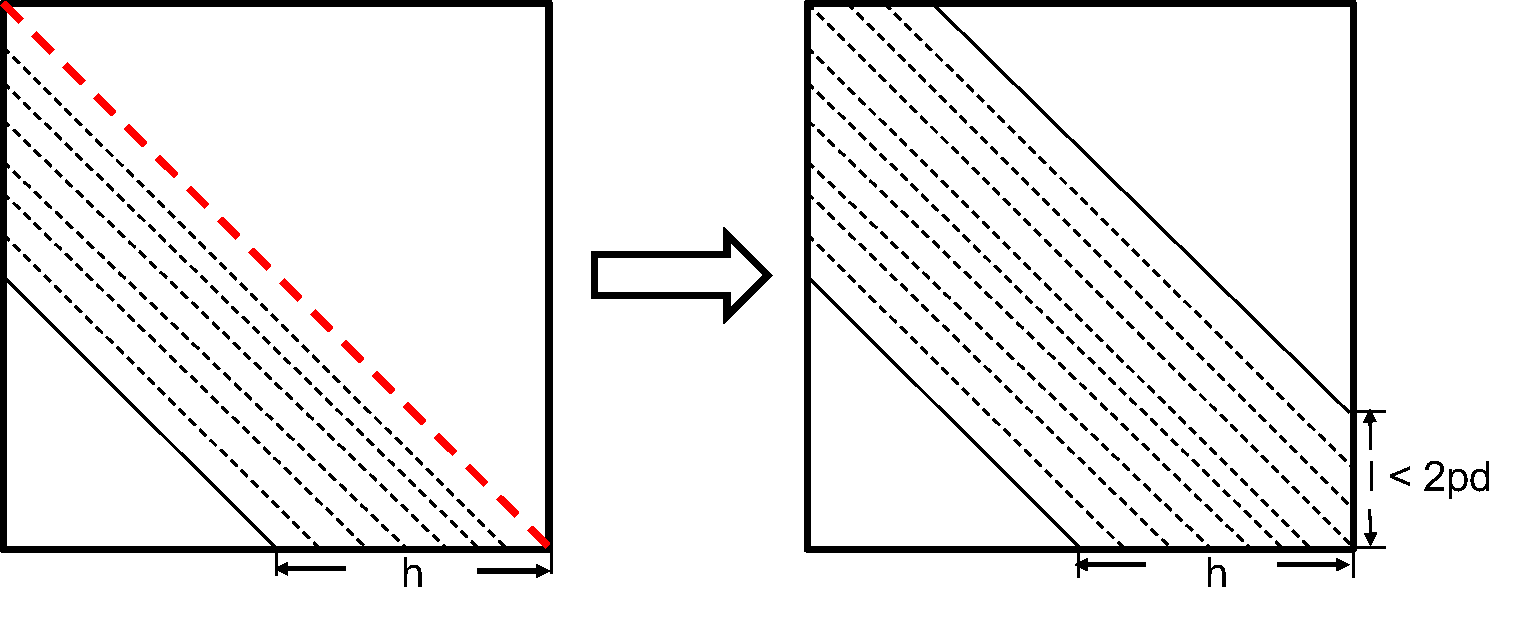
\includegraphics[width=5.8in]{fig/matgen.pdf}
	\caption{Matrix Generation. The left is the initial matrix $M_0$ with given spectrum on the diagonal, and the $h$ lower diagonals with random values; the right is the generated matrix $M_t$ with nilpotency matrix determined by the parameters $d$ and $p$.}
	\label{fig:matgen}
\end{figure}

\begin{algorithm*}[htbp]{}
	\caption{Matrix Generation Method}   
	\label{alg:matgen}   
	\begin{algorithmic}[1]
		\Function {matGen}{$input$:$Spec_{in} \in \mathbb{C}^n$, $h$, $d$, $output$: $M_t \in \mathbb{C}^{n\times n}$}
		\State Insert the entries in $h$ lower diagonals of $M_o \in \mathbb{N}^{n \times n}$
		\State Insert $Spec_{in}$ on the diagonal of $M_0$
		\State $M_0=(2d)!M_0$
		\State Generate nilpotent matrix $A \in \mathbb{C}^{n\times n}$ with selected parameters $d$ and $p$
		\For {\texttt{$i=0, \cdots, 2d-1$}}
		\State $M_{i+1}=M_i+(\prod_{k=i+1}^{2d}k)(\widetilde{A_A})^i(M_0)$
		\EndFor 
		\State $M_t = \frac{1}{(2d)!}M_{2d}$
		\EndFunction
	\end{algorithmic}
\end{algorithm*}

For $M_t$, if $M_0$ is a lower triangular matrix having $h$ non zero diagonals, it will be a band diagonal matrix, whose number of new diagonals in the upper triangular zone will be at most $2pd-1$. Thus the maximal number of the bandwidth of matrix $M_t$ is: $width = h + 2pd-1$, as in Fig. \ref{fig:matgen}. In general, researchers use these matrices to test the iterative methods of sparse linear systems. Thus after the generation of band matrix, it can be transferred to be sparse with the help of permutation matrices. Fig. \ref{fig:matgene} gives an example showing the pattern of the generated matrix by SMG2S. In general, researchers use these matrices to test the iterative methods for sparse linear systems. The $h$ lower diagonals of the initial matrix can set to be sparse, which ensures the sparsity of the final generated matrix, as shown in Fig. \ref{fig:matgene}. Moreover, the permutation matrix can also be applied to change the sparsity of the generated matrix further.

The operations complexity $C$ of Algorithm \ref{alg:matgen} is given as: 

\begin{equation}
\label{eq:serial time}
\begin{aligned}
%C=(2d^2+(5+2h)d+(3h-4))n+\frac{h(h+1)(2d+1)}{2}-2(d+2).
C\approx 2(2d^2+(4h-2)d-(h+5))n-h(h+1)(h+4d-4).
\end{aligned}
\end{equation}

In Equation (\ref{eq:serial time}), the complexity of SMG2S is $max(\mathcal{O}(hdn),\mathcal{O}(d^2n))$. The worst case would be an $\mathcal{O}(n^3)$ problem for operations with large $d$ and $h$, and it would require $\mathcal{O}(n^2)$ memory storage. But if we want to generate a band matrix with small bandwidth which means $d \ll n$ and $h \ll n$, it turns to be a $\mathcal{O}(n)$ problem with good potential scalability and to consume $\mathcal{O}(n)$ memory storage.

\begin{figure}[t]
	\centering
	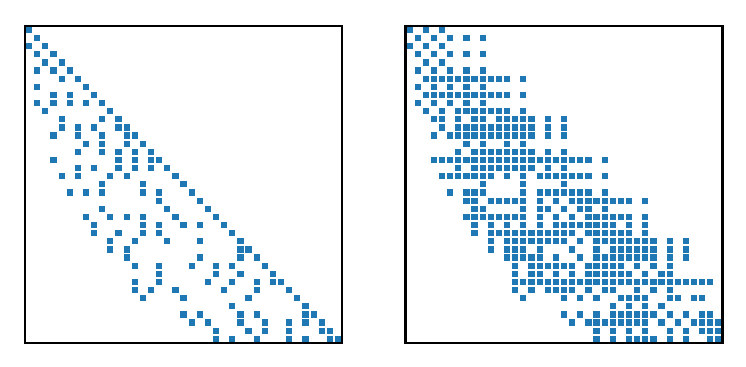
\includegraphics[width=5.2in]{fig/matgen/matgen.eps}
	\caption{Matrix Generation Pattern Example.}
	\label{fig:matgene}
\end{figure}

\section{Parallel Impementation and Evaluation}\label{Parallel Impementation and Evaluation}

In this section, we present the parallel implementation of SMG2S for homogeneous and heterogeneous clusters. The former is initially implemented based on MPI and PETSc, and the latter is based on MPI, CUDA, and PETSc. We select the mature library PETSc firstly since it provides several methods to verify the generated matrices, and also the basic operations inside are optimized for different computer architectures. After the validation of matrix generation based on PETSc, an open source parallel software with specific optimized communication is also implemented based on MPI and C++.

\subsection{Basic Implementation on CPUs}

For the initial CPU implementation, we chose PETSc instead of ScaLAPACK because we would like to evaluate the solvers for sparse linear systems. As shown in Algorithm \ref{alg:matgen}, the kernel of generation is the SpGEMM operation of $AM$ and $MA$, and the matrix-matrix addition (AYPX operation) as $AM-MA$. All the sparse matrices during the generation procedure are stored by the block CSR format which is provided in default by PETSc. We use the matrix operations supported by PETSc to facilitate the implementation. The block diagonal parallel matrix based on MPI are partitioned and stored into several submatrices. For example, if there are three MPI process: $proc1$, $proc2$ and $proc3$, the matrix can be divided into blocks as the Formula (\ref{parallelmat}). The submatrix $A$, $B$ and $C$ is stored in $proc1$,  $D$, $E$ and $F$ in $proc2$, and $G$, $H$ and $I$ is stored in $proc3$. On each process, the diagonal part and the off-diagonal are separately stored into two sequence block matrices. The parallel SpGEMM and AXPY operations for CPUs are already supported by PETSc \cite{balay2016petsc}. We use these functions directly to facilitate the implementation.


\begin{equation}
\label{parallelmat}
\left[
\begin{BMAT}(c)[4pt]{c|c|c}{c|c|c}
A  & B & C  \\
D & E & F  \\
G & H & I 
\end{BMAT}
\right]
\end{equation}


\subsection{Implementation on Multi-GPU}

\begin{figure}[t]
	\centering
	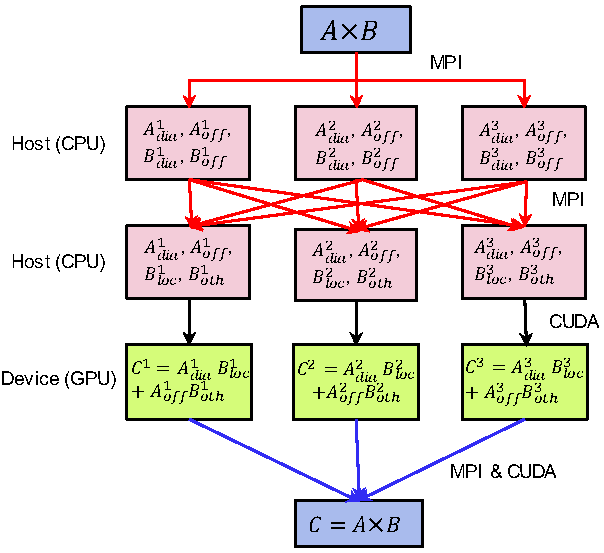
\includegraphics[width=5.4in]{fig/spgemm2.pdf}
	\caption{The structure of a CPU-GPU implementation of SpGEMM, where each GPU is attached to a CPU. The GPU is in charge of the computation, while the CPU handles the MPI communication among processes.}
	\label{fig:cuda}
\end{figure}

PETSc does not supply the SpGEMM and AXPY operations for GPU clusters. Thus we implemented them using MPI, CUDA and cuSPARSE library based on the PETSc data structure definitions. The structure of implementation is given in Fig. \ref{fig:cuda} which uses sparse matrix $A$ and $B$ multiplication as an example. Firstly, the same as in PETSc, $A$ and $B$ are divided into slices, and each slice is saved in a process. In each process of number $i$, the local matrices are all saved as two separate sequence matrix, noted as $A^i_{dia}$ and $A^i_{off}$ for matrix $A^i$, $B^i_{dia}$ and $B^i_{off}$ for matrix $B^i$. Then $B^i_{dia}$ and $B^i_{off}$ are combined together as a novel sequence matrix noted as $B^i_{loc}$ in each process $i$. With MPI functionalities, each CPU gather all the remote data of matrix $B$ from the other processes, and construct them to a new sequence matrix $B^i_{oth}$. These matrices from each process are copied to one attached GPU, and calculate $C^i=A^i_{dia}B^i_{loc}+A^i_{off}B^i_{oth}$. The matrix operations on each GPU device is supported by the cuSPARSE. The final result $C$ can be obtained by gathering all slices $C_i$ from all the devices.

\subsection{Communication Optimized Implementation with MPI}

The implementation of SMG2S, especially the parallel SpGEMM kernel's communication can be specifically optimized based on the particular property of nilpotent matrix $A$. In fact, $A$ can be determined by three parameters $p$, $d$ and $n$ that we have mentioned in Section \ref{Matrix_Generation_Method}, thus it is not necessary to explicitly implement this parallel matrix. We note this nilpotent matrix as $A(p,d,n)$. Denote that for any matrix $J$, $J(i,j)$ represents the entry in row $i$ and column $j$; $J(i,:)$ represents all the entries of row $i$; and $J(:,j)$ represents all the entries of column $j$. Then, we observe the effects of right and left-multiplying this nilopotent matrix $A(p,d,n)$ on a general matrix $M$ by basic mathematical matrix operations. As shown in Fig. \ref{fig:amma}, the right-multiplcation operation of $A(p,d,n)$ will shift all the entries of first $n-p$ columns to right side with an offset $p$. Denote $MA$ the result matrix gotten by the right-multiplying $A$ on $M$ (the result of $MA$ operation). We have $MA(:,j)=M(:,j-p), \forall j \in p,\cdots, n-1$, and $MA(:,j)=0,  \forall j \in 0,\cdots, p-1$. Similarly, the left-multiplying $A(p,d,n)$ on $M$ will shift the whole entries of last $n-p$ rows to up side with an offset $p$. Denote $AM$ the matrix gotten by the left-multiplying $A$ on $M$ (the result of $AM$ operation). We have $AM(i,:)=M(i+p,:), \forall i \in 0,\cdots, n-p-1$, and $AM(i:,)=0,  \forall i \in p,\cdots, n-1$. Moveover, the parameter $d$ decides that $MA(:,r(d+1))=0$ and $AM(r(d+1),:)=0$ with $r \in 1, \cdots, \lfloor \frac{n}{d+1}\rfloor$. 

\begin{figure}[t]
	\centering
	\subfloat[AM Operation.]{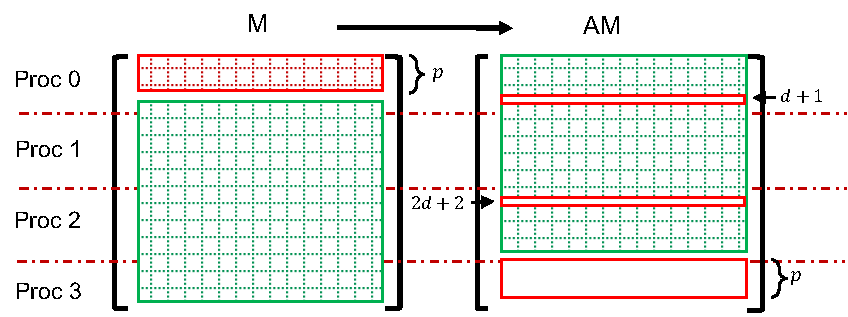
\includegraphics[width=6.3in]{fig/AM.pdf}%
		\label{am}}
	\\
	\subfloat[MA Operation.]{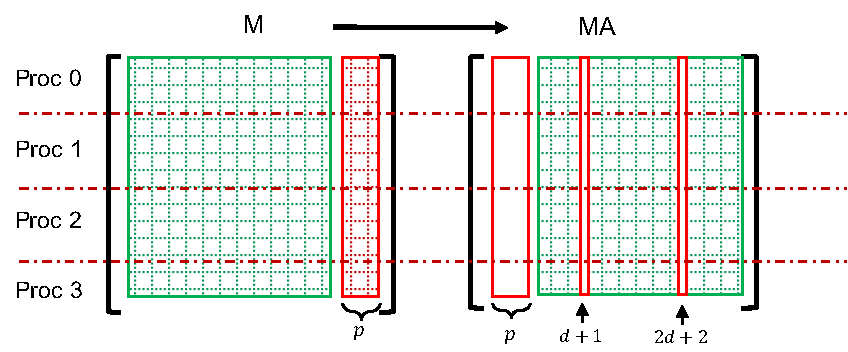
\includegraphics[width=6.3in]{fig/MA.pdf}%
		\label{ma}}
	\caption{AM and MA operations. }
	\label{fig:amma}
\end{figure}


When thinking about the implementation in parallel on distributed memory systems, the three integer parameters $p$, $d$ and $n$ can be shared by all MPI processes, and the parallel operations $AM$ and $MA$ are different from the general parallel SpGEMM, which is communication bounded. We analyze these two operations in Fig. \ref{fig:amma}. Firstly, the general matrix $M$  is one-dimensional distributed by row across $m$ MPI process. As shown in  Fig. \ref{ma}, for $MA$, there is no communication inter different MPI processes since the data are moved inside each row. Assume that $ \lfloor \frac{n}{m}\rfloor \geq p$, for $AM$, the intercommunication of MPI takes place when the MPI process $k$ ($k \in 1, \cdots, m-1$) should send the first $p$ rows of their sub-matrix to the closest previous MPI process numbering $k-1$. The communication complexity for each process is $\mathcal{O}(np)$. When generating the band matrix with low bandwidth $b$, it tends to be a $\mathcal{O}(bp)$ with $p=1$ or $2$. The MPI-based optimization implementations of AM and MA are respectively given by Algorithm \ref{alg:am} and \ref{alg:ma}. The communication inter MPI process is assumed by the asynchronous sending and receiving functions. In this algorithm, $M_k$, $MA_k$ and $AM_k$ imply the sub-matrices on process $k$ with $t$ rows. The rows and columns of these sub-matrices in Algorithm \ref{alg:am} and \ref{alg:ma} are all indexed by the local indices.

\begin{algorithm}[t]{}
	\caption{Parallel MPI AM Implementation}   
	\label{alg:am}   
	\begin{algorithmic}[1]
		\Function {AM}{$input$: matrix $M$, matrix row number $n$, $p$, $d$, proc number $m$; $output$: matrix $AM$}
		\State Distribute $t$ row blocks $M_k$ of $M$ to MPI process $k$
		\For {$p+1 \leq i < t $}
		\For {$0 \leq j < n$}
		\If{$M(i,j) \neq 0$}
		\State $AM_k(i-p,j) = M_k(i,j)$
		\EndIf
		\EndFor
		\EndFor
		\For {$0 \leq i < p $}
		\If {$k \neq 0$}
		\State $isend$ $ith$ $row$ $M_k(i)$ to $k-1$
		\EndIf
		\If {$k \neq m-1$}
		\State $irecv$ $ith$ $row$ $M_k(i)$ from $k+1$
		\State $AM_k(t-p+i)=M_k(i)$
		\EndIf
		\EndFor
		\EndFunction
		
	\end{algorithmic}  
	
\end{algorithm}

The communication-optimized SMG2S is implemented based on MPI and C++. The submatrix on each process is stored in ELLPACK format, using the key-value map containers provided by C++. The key-value map implementation facilitates the indexing and moving of the rows and columns. We did not implement a GPU version of SMG2S with this kind of communication since its core is the data movement among different computing units, which is not well suitable for multi-GPU architecture.


\begin{algorithm}[t]{}
	\caption{Parallel MPI MA Implementation} 
	\label{alg:ma}   
	\begin{algorithmic}[1]
		\Function {MA}{$input$: matrix $M$, matrix row number $n$, $p$, $d$, proc number $m$; $output$: matrix $MA$}
		\State Distribute $t$ row blocks $M_k$ of $M$ to process $k$ 
		\For {$0 \leq i < t $}
		\For {$p+1 \leq j < n$}
		\If{$M_k(i,j) \neq 0$}
		\State $MA_k(i,j+p) = M_k(i,j)$
		\EndIf
		\EndFor
		\EndFor 
		\EndFunction
	\end{algorithmic} 
	
\end{algorithm}

\section{Parallel Performance Evaluation}\label{Parallel Performance Evaluation}
\subsection{Hardware}
In experiments, we implement SMG2S on the supercomputers \textit{Tianhe-2} and \textit{Romeo}. \textit{Tianhe-2} system has been six times No.1 in the Top500 list, which is installed at the National Super Computer Center in Guangzhou of China. It is a heterogeneous system made of Intel Xeon CPUs and Intel Knights Corner (KNC), with 16000 compute nodes in total. Each node composes 2 Intel Ivy Bridge 12 cores @ 2.2 GHz. \textit{Romeo} is located at University of Reims Champagne-Ardenne, France. It is also a heterogeneous system made of Xeon CPUs and Nvidia GPUs, with 130 BullX R421 nodes. Each node composes 2 Intel Ivy Bridge 8 cores @ 2.6 GHz and 2 NVIDIA Tesla K20x GPUs. In this article, we do not test SMG2S using the KNC on \textit{Tianhe-2} since our parallel implementation does not support it with good performance.
\subsection{Strong and Weak Scalability Evaluation}

\begin{table}[htbp]
	\centering
	\caption{Details for weak scaling and speedup evaluation.}
	\renewcommand{\arraystretch}{1.5}
	\small
	\subfloat[Subtable 1 list of tables text][Matrix size for the CPU weak scaling tests on $Tianhe$-2.]{
		\begin{tabular}{x{2.6cm}|x{1.4cm}|x{1.4cm}|x{1.4cm}|x{1.4cm}|x{1.4cm}|x{1.4cm}}
			\toprule
			\cellcolor{gray!50}CPU number & \cellcolor{gray!50}48 & \cellcolor{gray!50}96 & \cellcolor{gray!50}192 & \cellcolor{gray!50}384 & \cellcolor{gray!50}768 & \cellcolor{gray!50}1536\\
			\midrule
			matrix size & $1\times10^6$ & $2\times10^6$  & $4\times10^6$  & $8\times10^6$  & $1.6\times10^7$  & $3.2\times10^7$ \\
			\bottomrule
	\end{tabular}}
	\qquad
	\subfloat[Subtable 2 list of tables text][Matrix size for the CPU weak scaling on $ROMEO$.]{
		\begin{tabular}{x{2.6cm}|x{1.5cm}|x{1.5cm}|x{1.5cm}|x{1.5cm}|x{1.5cm}}
			\toprule
			\cellcolor{gray!50}CPU number & \cellcolor{gray!50}16 & \cellcolor{gray!50}32 & \cellcolor{gray!50}64 & \cellcolor{gray!50}128 & \cellcolor{gray!50}256\\
			\midrule
			matrix size & $4\times10^5$ & $8\times10^5$ & $1.6\times10^6$ & $3.2\times10^6$ & $6.4\times10^6$\\
			\bottomrule
	\end{tabular}}
	
	\subfloat[Subtable 3 list of tables text][Matrix size for the GPU weak scaling and speedup evaluation on $ROMEO$.]{
		\begin{tabular}{x{3.8cm}|x{1.4cm}|x{1.4cm}|x{1.4cm}|x{1.4cm}|x{1.4cm}}
			\toprule
			\cellcolor{gray!50}CPU or GPU number & \cellcolor{gray!50}16 & \cellcolor{gray!50}32 & \cellcolor{gray!50}64 & \cellcolor{gray!50}128 & \cellcolor{gray!50}256\\
			\midrule
			matrix size &$2\times10^5$ & $4\times10^5$ & $8\times10^5$ & $1.6\times10^6$ & $3.2\times10^6$\\
			\bottomrule
	\end{tabular}}
	\label{table:matrixsize}
\end{table}

In this section, we will use double-precision real and complex values to evaluate the strong and weak scalability of SMG2S's different implementations on CPU and multiple GPUs. All the test matrices in this paper are generated with the $h$ set to be $10$  and $d$ to be $7$. The details of the weak scaling experiments are given in Table \ref{table:matrixsize}. The matrix size of the strong scaling experiments on $Tianhe-2$ with CPUs, $ROMEO$ with CPUs and $ROMEO$ with GPUs are respectively $\num[round-precision=2,round-mode=figures]{16000000}$, $\num[round-precision=2,round-mode=figures]{3200000}$ and $\num[round-precision=2,round-mode=figures]{800000}$. The results are given in Fig. \ref{fig:scaling-cpu-tianhe-2}, Fig. \ref{fig:scaling-cpu-romeo} and Fig. \ref{fig:scaling-gpu-romeo}. The weak scaling for the PETSc implementation of SMG2S on \textit{Tianhe-2} trends to be bad when MPI processes number is larger than $768$, where the communication overhead becomes dominant for computation. But for the communication optimized SMG2S, both the strong and weak scaling perform well when the MPI process number is larger than $768$. The experiments show that SMG2S implemented with GPUs can still have good strong and weak scalability. In conclusion, SMG2S has always good strong scaling performance when $d$ and $h$ are much smaller than the dimension of the matrix $n$, because it turns to be a $\mathcal{O}(n)$ problem. The weak scalability is good enough for most cases. The reason is that the nilpotent matrix $A$ in SpGEMM is simple with not many non-zero elements. Therefore there is not enormous communication among different computing units. The weak scalability has its drawback in case that the computing unit number come to be huge for the SMG2S implementation based on PETSc, where the communication overhead become dominant. The specific implementation of communication-optimized SMG2S makes his strong and weak scalability better. It is also shown that the double precision complex type matrix generation takes almost two times time over the double precision real type for the basic SMG2S implementation, but the time consumption of complex and real type matrix generation of optimized SMG2S seems similar. The reason is that there is no numerical values multiplication anymore in the optimized implementation of SMG2S. 

\begin{figure}[htbp]
	\centering
	\subfloat[CPU strong scaling on Tianhe-2.]{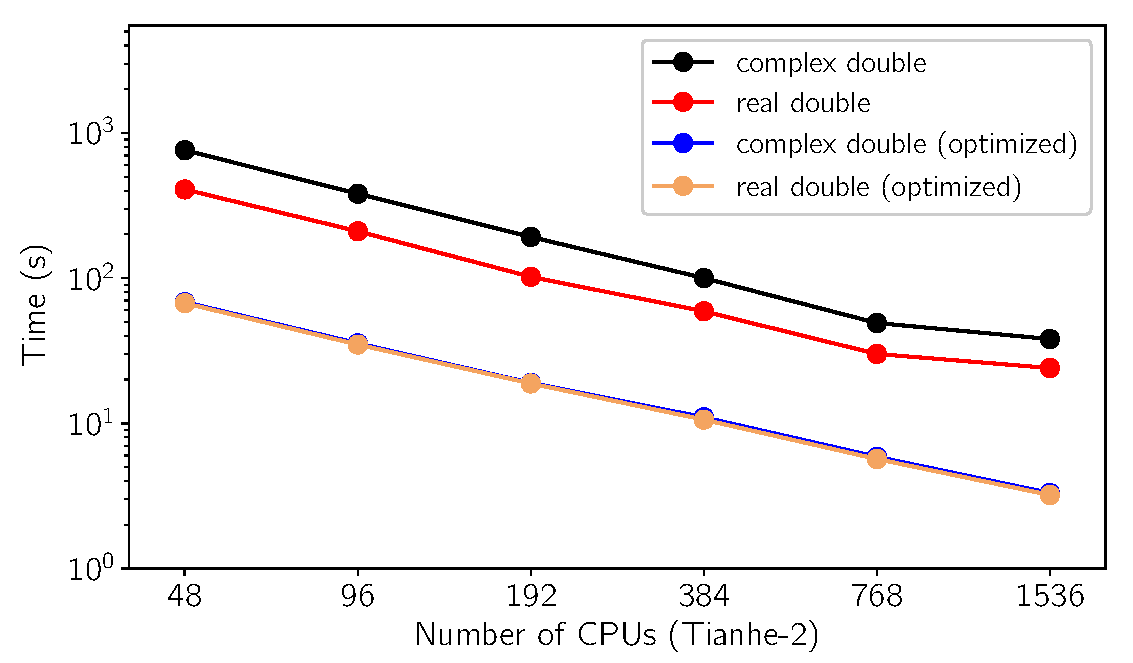
\includegraphics[width=0.499\linewidth]{fig/matgen/cpu_th2_strong_scalable.eps}%
		\label{ss_tianhe}}
	\subfloat[CPU weak scaling on Tianhe-2.]{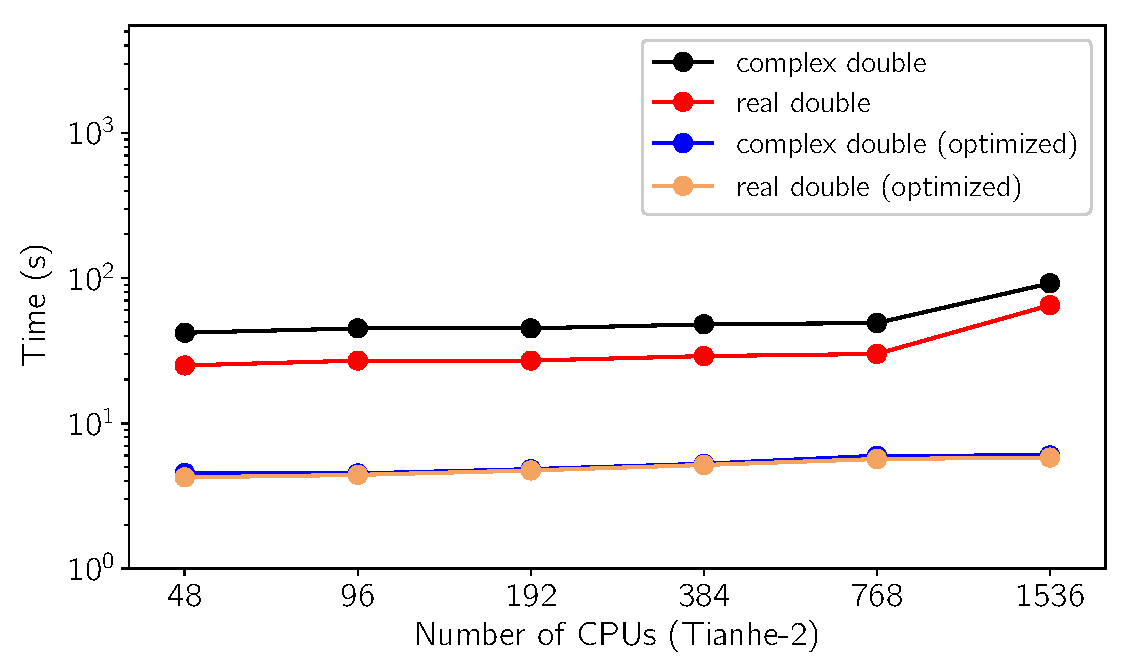
\includegraphics[width=0.499\linewidth]{fig/matgen/cpu_th2_weak_scalable.eps}%
		\label{ws_tianhe}}
	\caption{Strong and weak scaling results of SMG2S on Tianhe-2. A base 2 logarithmic scale is used for X-axis, and a base 10 logarithmic scale for Y-axis. }
	\label{fig:scaling-cpu-tianhe-2}
\end{figure}

\begin{figure*}[htbp]
	\centering
	\subfloat[CPU strong scaling on ROMEO.]{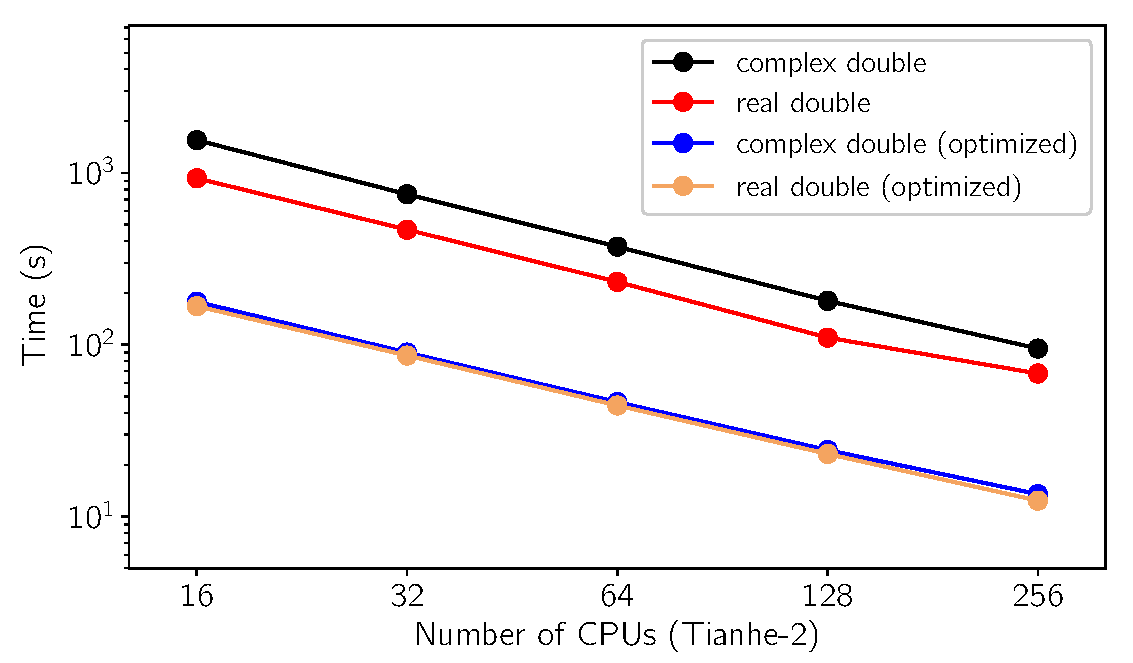
\includegraphics[width=0.499\linewidth]{fig/matgen/cpu_romeo_strong_scalable.eps}%
		\label{romeo}}
	\subfloat[CPU weak scaling on ROMEO.]{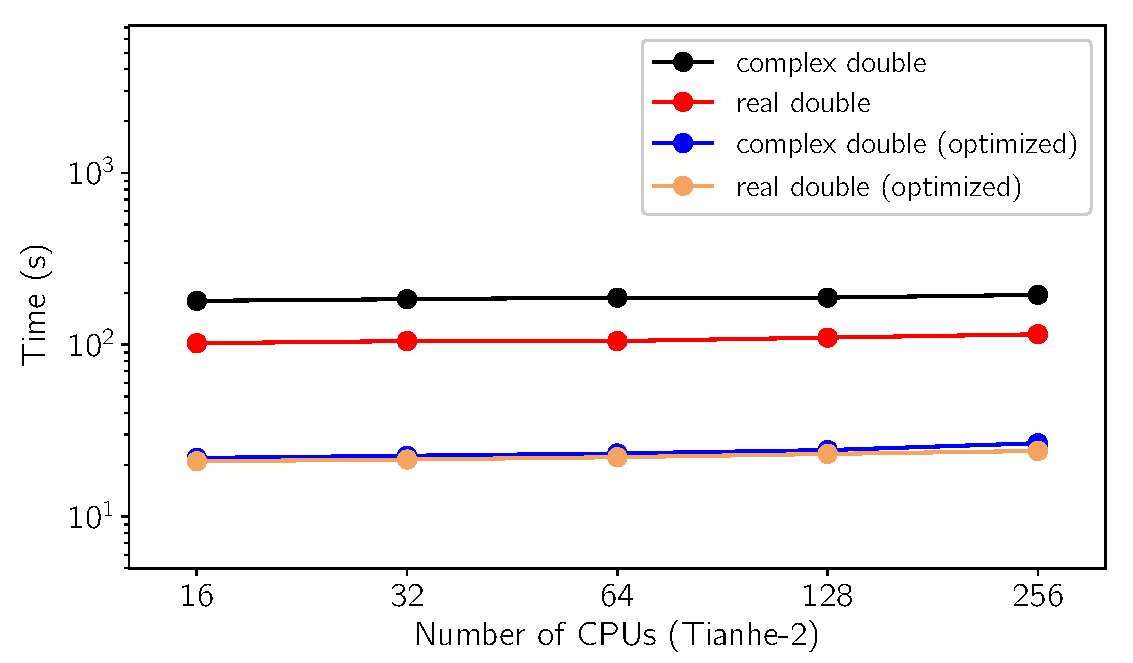
\includegraphics[width=0.499\linewidth]{fig/matgen/cpu_romeo_weak_scalable.eps}%
		\label{romeo_gpu}}
	\caption{Strong and weak scaling results of SMG2S on ROMEO. A base 2 logarithmic scale is used for X-axis, and a base 10 logarithmic scale for Y-axis. }
	\label{fig:scaling-cpu-romeo}
\end{figure*}

\begin{figure*}[t]
	\centering
	\subfloat[GPU strong scaling on ROMEO.]{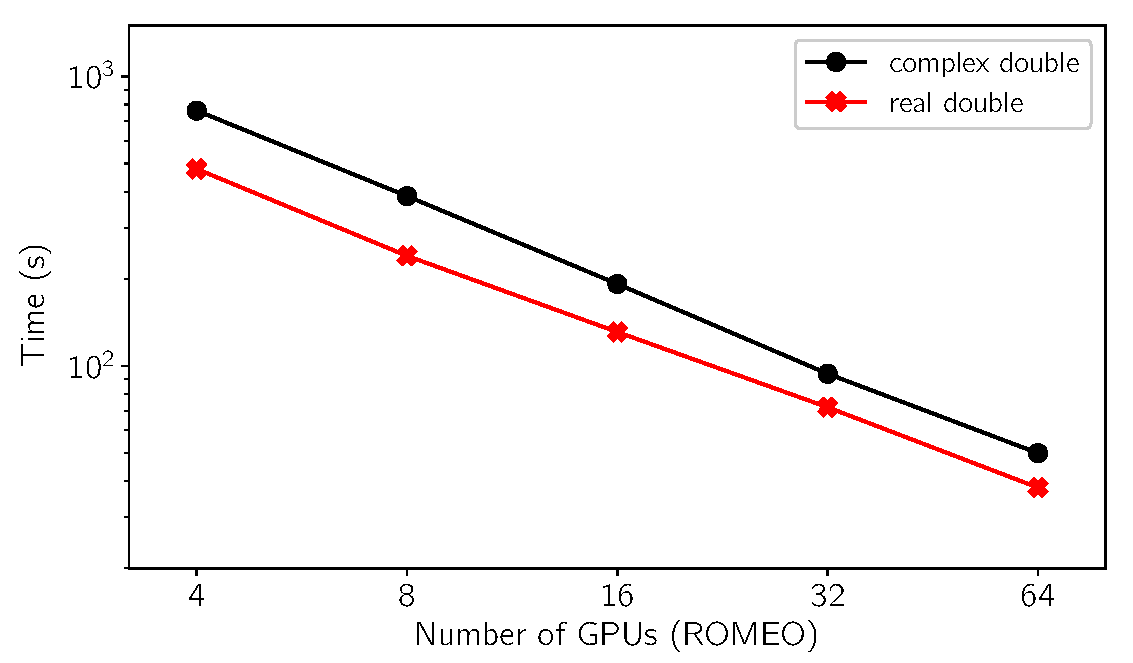
\includegraphics[width=0.499\linewidth]{fig/matgen/gpu_strong_scalable.eps}%
		\label{ss_romeo_gpu}}
	\subfloat[GPU weak scaling on ROMEO.]{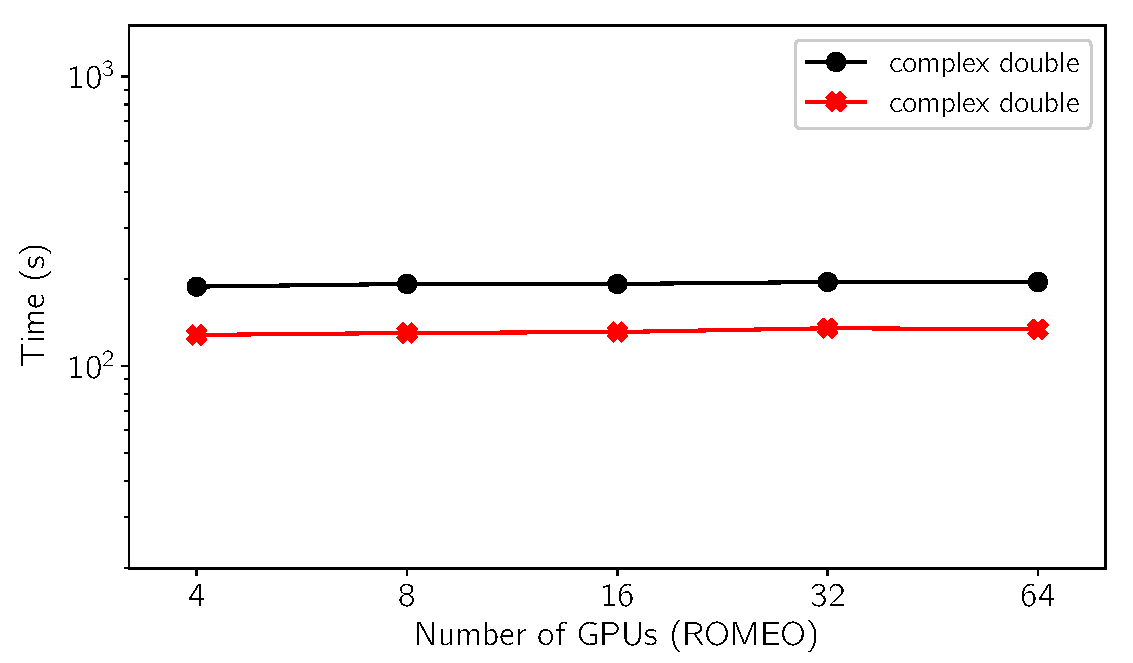
\includegraphics[width=0.499\linewidth]{fig/matgen/gpu_weak_scalable.eps}%
		\label{ws_romeo_gpu}}
	\caption{Strong and weak scaling results of SMG2S on ROMEO with multi-GPUs. A base 2 logarithmic scale is used for X-axis, and a base 10 logarithmic scale for Y-axis. }
	\label{fig:scaling-gpu-romeo}
\end{figure*}

\begin{figure*}[t]
	\centering
	\hfil
	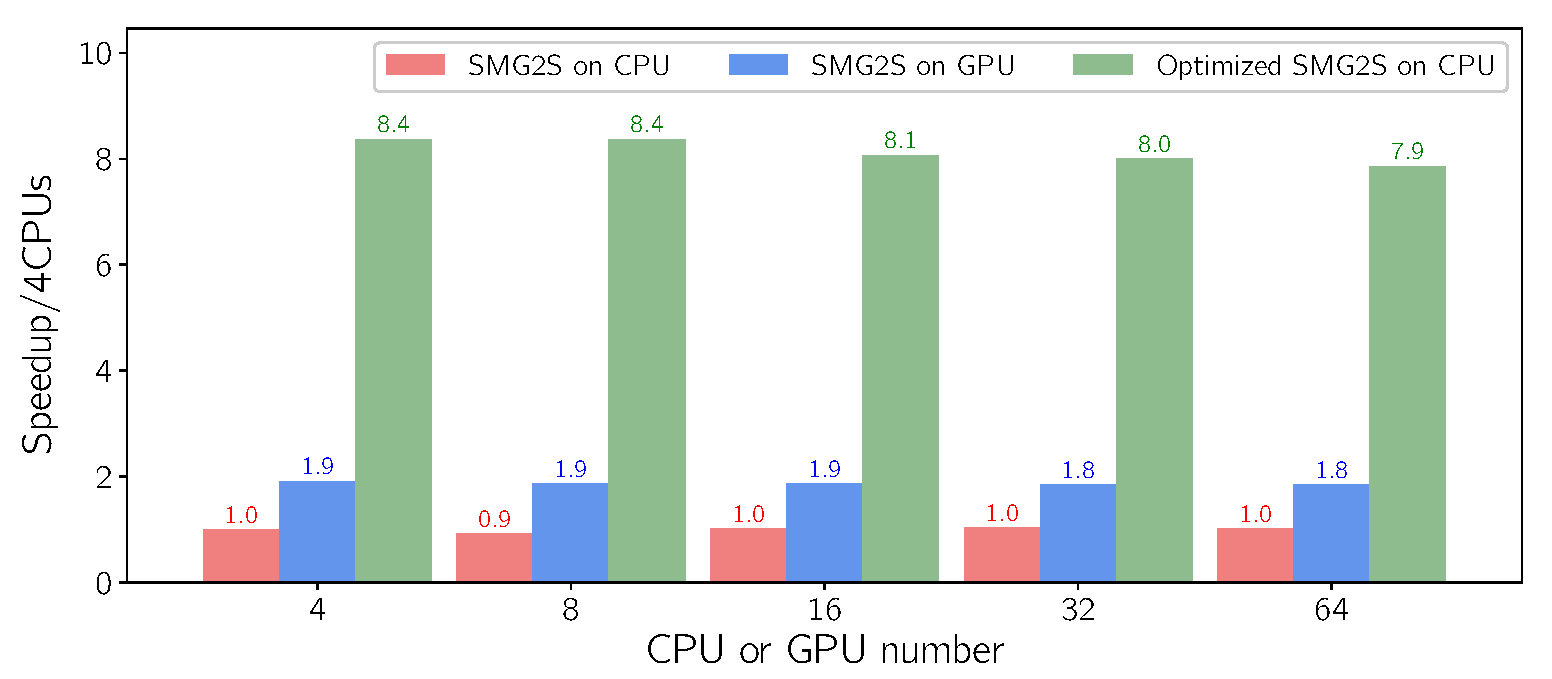
\includegraphics[width=0.99\linewidth]{fig/matgen/speedup.eps}%
	\caption{Weak scaling speedup comparison of GPUs on ROMEO.}
	\label{speedup}
\end{figure*}

\subsection{Speedup Evaluation}

The speedup of both SMG2S on multi-GPU and communication-optimized SMG2S on the CPUs compared with the PETSc-based implementation on CPU are also tested on \textit{Romeo}. According to the previous evaluation that complex and real value types always have good scalability, we select the double precision complex values for the speedup evaluation. The details of experiments are also given in Table \ref{table:matrixsize}c. The results are shown in Fig. \ref{speedup}. We can find that the GPU version of SMG2S has almost $1.9\times$ speedup over the PETSc CPU version. The communication-optimized SMG2S on CPUs has about $8\times$ speedup over the basic PETSc CPU version.

\subsection{Performance Analysis}

In conclusion, SMG2S always has good strong scalability when $d$ and $h$ are much smaller than the dimension of the matrix to be generated $n$, because It turns to be a $\mathcal{O}(n)$ problem. The weak scalability is good enough for most cases. The reason is that the matrices dealt with in SpGEMM are simple with not many non-zero elements. Therefore there are not enormous communication among different computing units. The weak scalability has its drawback in case that the computing unit number come to be huge for the SMG2S implementation based on PETSc, where the communication overhead become dominant. The strong and weak scaling for communication optimized SMG2S is good with its special implementation. It is also shown that the double-complex type matrix generation takes almost two times time over the double-real type for the basic SMG2S implementation. The time consumption of complex and real type matrix generation of optimized SMG2S seems similar. The reason is that in the optimized implementation of SMG2S, there are not numerical values multiplication anymore.  It also has the capacity to take advantage of GPUs to accelerate the computation with about $1.9$x speedup than CPUs. The communication optimized version has $8$x speedup over the basic implementation.

\section{Verification Method}\label{Verification Method}

In the last section, we show the good parallel performance of SMG2S, and then it is necessary to verify if the generated matrices are able to keep the given spectra with enough accuracy. Generally, the iterative eigenvalue solvers such as the Arnoldi or other Krylov methods (\cite{petiton1992parallel}) are applied to approximate the dominant eigenvalues. However, the accuracy verification is an opposite case. Now there exists a value, and we want to check if it is an eigenvalue of a given matrix. These iterative methods cannot directly and efficiently deal with this kind of verification. In this section, we present a method for accuracy verification using the Shifted Inverse Power method, which was easily implemented in parallel.

\begin{algorithm}[t]{}
	\caption{Shifted Inverse Power method}   
	\label{alg:inversePower}   
	\begin{algorithmic}[1]
		\Function {sipm}{$input$: Matrix $A$, initial guess for desired eigenvalue $\sigma$, initial vector $v_0$, $output$: Approximate eigenpair ($\theta$, $v$)}
		\State $y=v_0$
		\For {\texttt{$i=1,2,3 \cdots$}}
		\State $\theta=||y||_\infty$
		\State $v=y/\theta$
		\State Solve $(A-\sigma I)y=v$
		\EndFor 
		\EndFunction
	\end{algorithmic}  
\end{algorithm}

\begin{figure}[t]
	\centering
	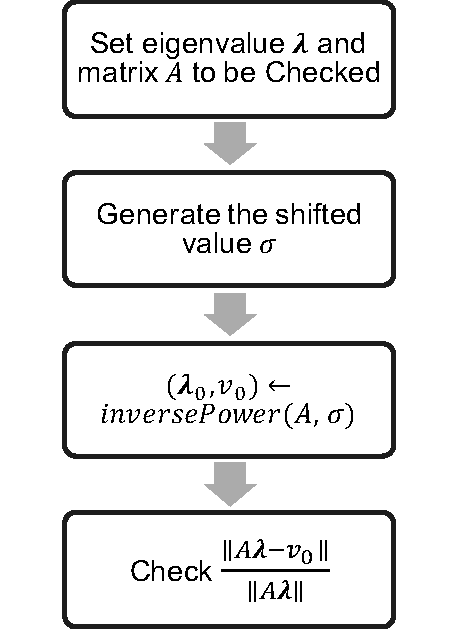
\includegraphics[width=0.4\linewidth]{fig/smg2s-check.pdf}
	\caption{SMG2S verification workflow.}
	\label{smg2s-check}
\end{figure}

The Power method is an algorithm to approximate the greatest eigenvalue. Meanwhile, the Inverse Power method is a similar iterative algorithm to find the smallest eigenvalue. The middle eigenvalues can be obtained by the Shifted Inverse Power method (\cite{hernandez2005single}).  This method is given in Algorithm \ref{alg:inversePower}. Its operation complexity is $\mathcal{O}(n^3)$. The Shifted Inverse Power method is used to compute the eigenvalue which is the nearest one to a given value in a few steps of iterations. The related eigenvector can be easily calculated by its definition and used to check if this given value is an eigenvalue of the matrix.

In details, for checking if the given value $\lambda$ is the eigenvalue of a matrix, we select a shifted value $\sigma$ which is close enough to $\lambda$. An eigenpair $(\lambda', v')$ with the relation $Av'=\lambda' v'$ can be approximated in very few steps by Shifted Inverse Power method, with $\lambda'$ is the closest eigenvalue to $\sigma$. Since $\sigma$ is very close to $\lambda$, it should be that $\lambda$ and $\lambda'$ are the same eigenvalue of a system, and $v'$ should be the eigenvector related to $\lambda$. In reality, even if the computed eigenvalue is very close to the true one, the related eigenvector may be quite inaccurate. For the right eigenpairs, the formula $Av'\approx\lambda v'$ should be satisfied. Based on this relation, we define the relative error as Formula (\ref{check}) to quantify the accuracy. 

\begin{equation}
\label{check}
error=
\frac{||Av'-\lambda v'||}{||Av'||}
\end{equation}

If $\lambda' = \lambda$, this $error$ should be $0$, if not, this generated matrix do not have an exact eigenvalue as $\lambda$. In real experiments, the exact solution cannot always be guaranteed with the arithmetic rounding errors of floating operations during the generation. A threshold could be set for accepting it or not.

\begin{table}[htbp]
	\renewcommand{\arraystretch}{1.4}
	\small	
	\caption{Accuracy Verification Results.}
	\label{accuracy}
	\centering
	\begin{tabular}{c|c|c|c|c}
		\toprule
		\cellcolor{gray!50}Matrix $N^{o}$& \cellcolor{gray!50}Size & \cellcolor{gray!50}Spectra & \cellcolor{gray!50}Acceptance (\%) & \cellcolor{gray!50}max $error$ \\
		\midrule
		1  & 100 & $Spec1$ &93&\num[round-precision=2,round-mode=figures]{0.02}\\
		\cellcolor{gray!20}2 & \cellcolor{gray!20}100 & \cellcolor{gray!20}$Spec2$   & \cellcolor{gray!20}94&\cellcolor{gray!20}\num[round-precision=2,round-mode=figures]{0.03}\\
		3 & 100 & $Spec3$  &100&\num[round-precision=2,round-mode=figures]{0.00007}\\
		\cellcolor{gray!20}4 & \cellcolor{gray!20}100 & \cellcolor{gray!20}$Spec4$  &\cellcolor{gray!20}100&\cellcolor{gray!20}\num[round-precision=2,round-mode=figures]{0.0000003}\\
		5 & 100 & $Spec5$  &100&\num[round-precision=2,round-mode=figures]{0.0000001}\\
		\bottomrule
	\end{tabular}
\end{table}

\subsection{Experimental Results}

In the experiments, we test the accuracy of SMG2S with five selected cases among the various tests of different spectral distributions. Fig. \ref{fig_first_case} and Fig. \ref{fig_third_case} are cases of clustered eigenvalues with different scales. Fig. \ref{fig_second_case} is a special case with the dominant part of eigenvalues clustered in a small region. Fig. \ref{fig_forth_case} is a case that composes the conjugate and closest pair eigenvalues. Fig. \ref{fig_first_case} is a case with discret distribution of eigenvalues in the complex plain. These figures compare the difference between the given spectra (noted as initial eigenvalues in the figures) and the approximated ones (noted as computed eigenvalues) by the Shifted Inverse Power Method. Clearly, the matrices generated by SMG2S can keep almost all the given eigenvalues in the four cases even they are very clustered and close. The acceptance threshold is set to be $1.0\times 10^{-3}$.

This acceptance for cases of Fig. \ref{fig_first_case}, Fig. \ref{fig_second_case}, Fig. \ref{fig_third_case}, Fig. \ref{fig_forth_case} and Fig. \ref{fig_fifth_case} are respectively 93\%, 94\%, 100\%, 100\% and 100\%. The maximum $error$ for them are respectively \num[round-precision=2,round-mode=figures]{0.02}, \num[round-precision=2,round-mode=figures]{0.03}, \num[round-precision=2,round-mode=figures]{0.00007}, \num[round-precision=2,round-mode=figures]{0.0000003} and \num[round-precision=2,round-mode=figures]{0.0000001}.  After the tests, we conclude that SMG2S is able to keep accurately the given spectra even for the very clustered and closest eigenvalues. In some cases, a very little number of too clustered eigenvalues may result in the inaccuracy of given ones, but in general, the generated matrix can fufil the need to evaluate the linear system and eigenvalue solvers. 

\begin{figure}[t]
	\centering
	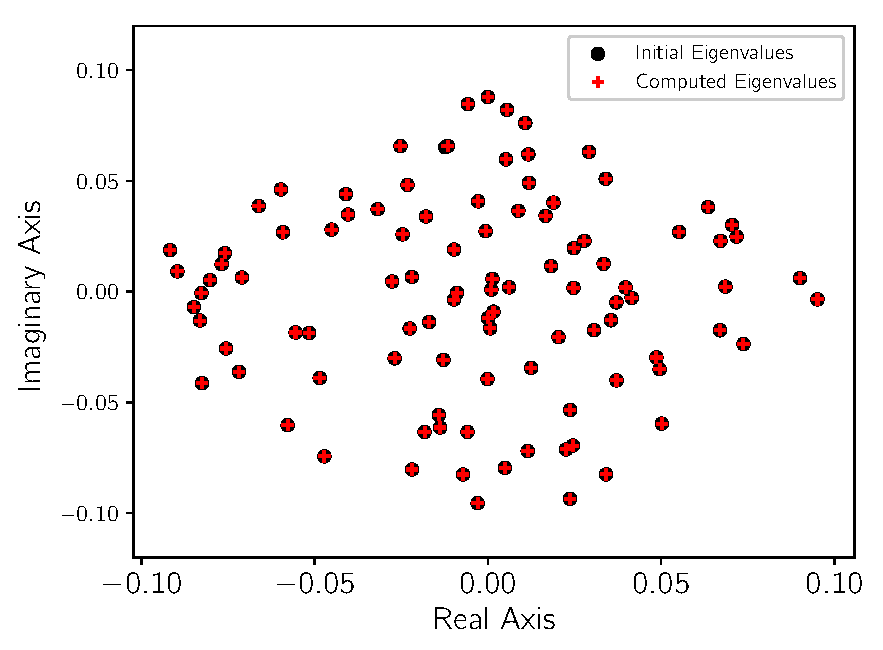
\includegraphics[width=5.8in]{fig/matgen/vector3.eps}
	\caption{Spec1: Clustered Eigenvalues I.}
	\label{fig_first_case}
\end{figure}

\begin{figure}[htbp]
	\centering
	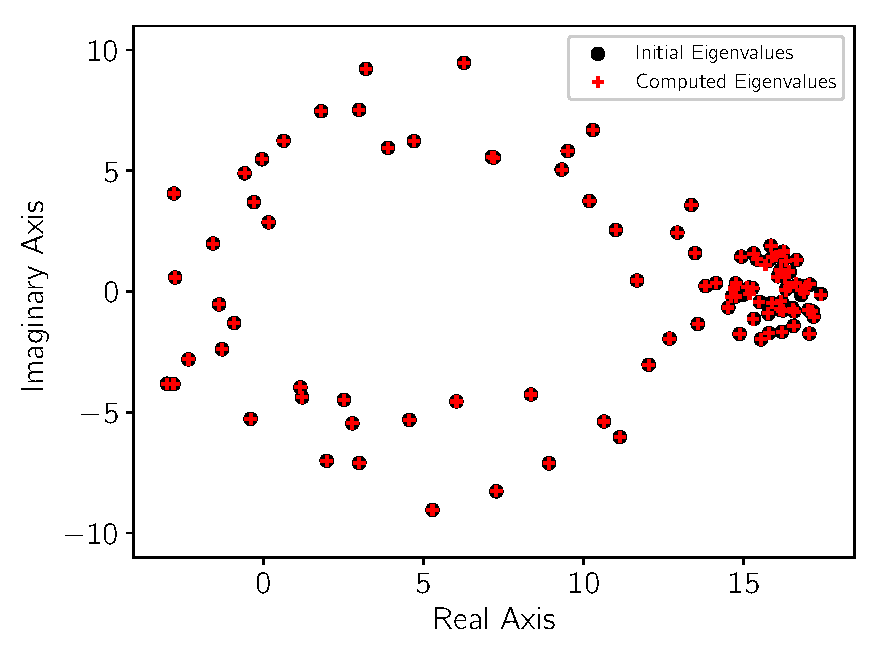
\includegraphics[width=5.8in]{fig/matgen/vector2.eps}
	\caption{Spec2: Clustered Eigenvalues II.}
	\label{fig_second_case}
\end{figure}

\begin{figure}[htbp]
	\centering
	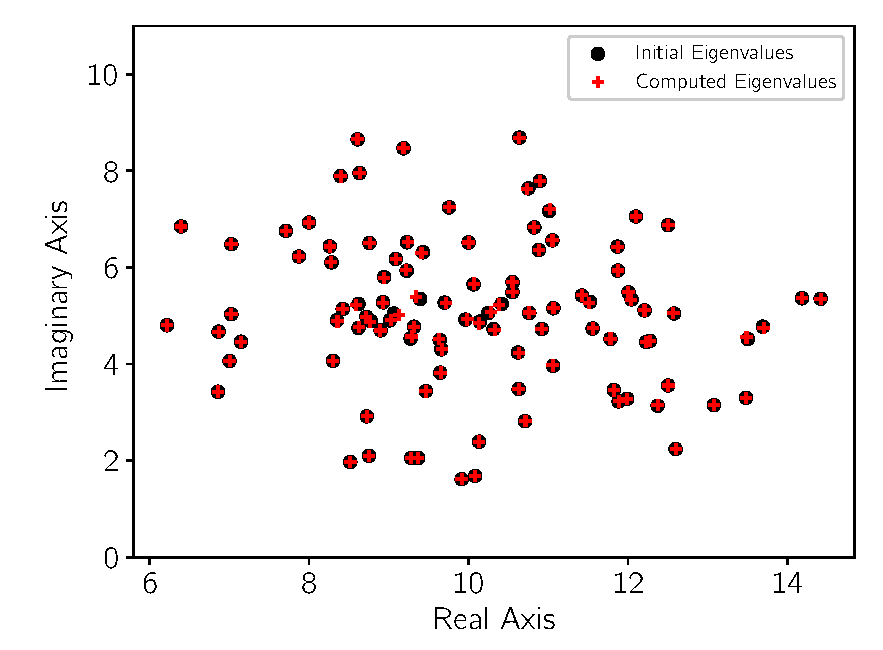
\includegraphics[width=5.8in]{fig/matgen/vector1.eps}
	\caption{Spec3: Clustered Eigenvalues III.}
	\label{fig_third_case}
\end{figure}


\begin{figure}[htbp]
	\centering
	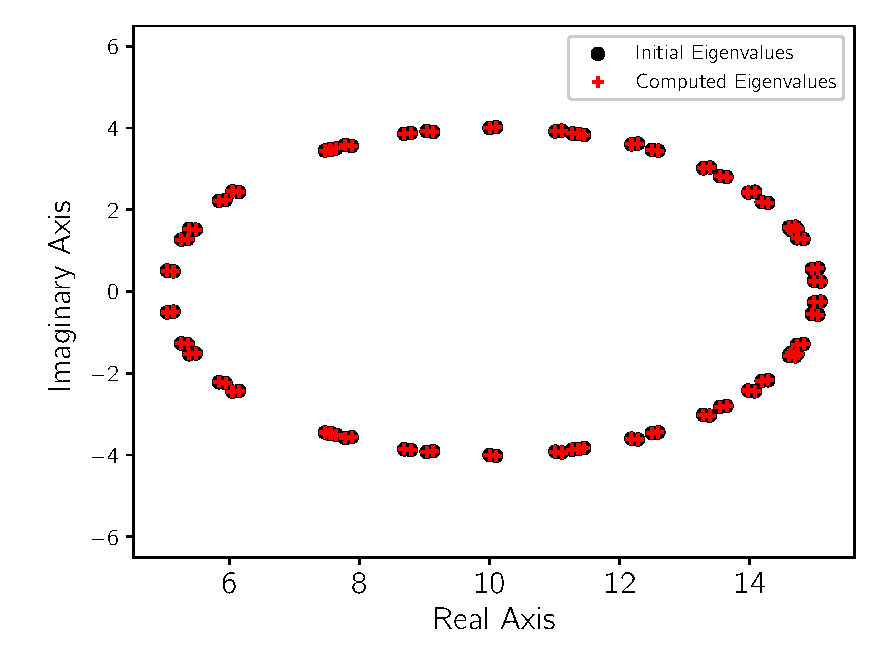
\includegraphics[width=5.8in]{fig/matgen/vector5.eps}
	\caption{Spec4: Conjugate and Closest Eigenvalues.}
	\label{fig_forth_case}
\end{figure}

\begin{figure}[htbp]
	\centering
	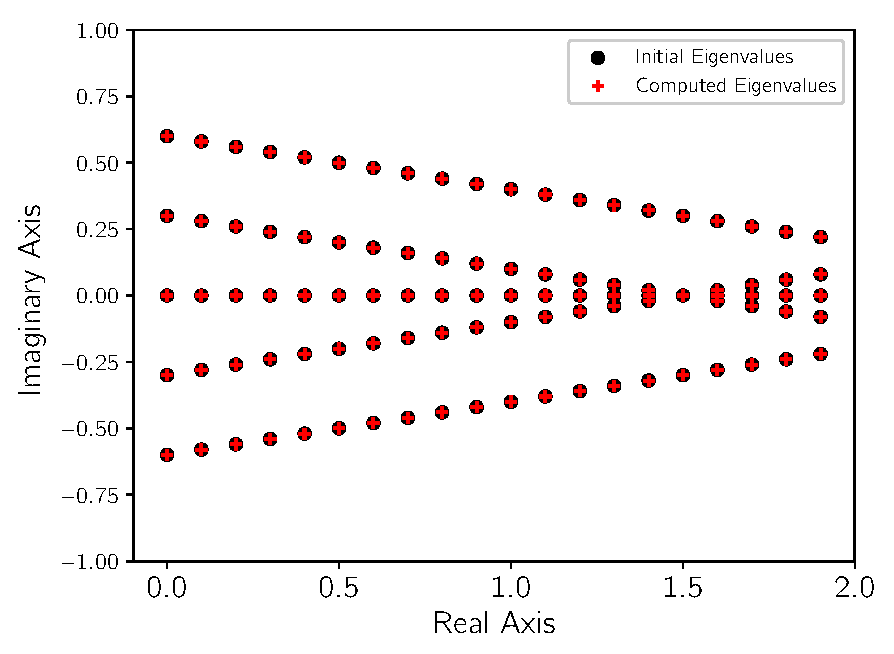
\includegraphics[width=5.8in]{fig/matgen/vector4.eps}
	\caption{Spec5: Distributed Eigenvalues.}
	\label{fig_fifth_case}
\end{figure}

\subsection{Arithmetic Precision Analysis}

Any floating operations will introduce rounding errors, which cannot be ignored for the generation of large matrices. Regarding the non-Hermitian matrix, its eigenvalues may be extremely sensitive to perturbation. This sensibility is bounded by \[bound(\lambda) \leq ||E||_2Cond(\lambda),\] with $Cond(\lambda)$ the condition number of related eigenvalue $\lambda$ and $||E||_2$ the Euclidean norm of errors \cite{saad2011numerical}. $Cond(\lambda)=1$ for the Hermitian matrices, but for the non-Hermitian ones, it can be excessively high. There are two solutions facing this problem. The first one is to ensure the eigenvalue to be well-conditioned. The second is to use the integer value for the matrix generation, since only integers and the operations $+$, $-$, and $\times$ on the microprocessor can make absolutely exact computations. As shown in Algorithm \ref{alg:matgen}, most of the operations in SMG2S are $+$, $-$ and $\times$, except the step 8 with a division operation. Without step 8, we could introduce a special SMG2S fully using integers to avoid the risks of rounding errors. The spectra of the generated matrix will be $(2d)!$ times of the given one. Moreover, the upper band's width of generated depends on the parameter $d$. The factorial of $2d$ can easily reach the limit of integer, even with unsigned long long type. Thus a special factorial function using multiple integers should be implemented in order to enlarge the upper band's width.

\section{Package, Interface and Application}\label{Package, Interface and Application}

SMG2S is packaged and released as an open source software based on MPI and C++. In this section, we present the package information of SMG2S and its interface to various programming languages and scientific computational libraries firstly. More details of the package can be found in the related manual \cite{wu2018smg2s}. Then, we give an example which uses SMG2S to evaluate different Krylov solvers. 

\subsection{Package}

\subsubsection{Installation Prerequisites}

Before the use of SMG2S, the below packages and libraries should be available on the computer platforms:

\begin{enumerate}[label=(\arabic*)]
	\item C++ Comiler with c++11 support;
	\item MPI;
	\item CMake (version minimum 3.6);
	\item (Optional) PETSc and SLEPc are necessary for the verification of accuracy of generated matrices to keep the given spectra.
\end{enumerate}

\subsubsection{Functions}

SMG2S provides the following subsets of functions, including the setup of parallel matrix and vector, the construction of particular nilpotent matrix, the matrix generation function, the interfaces to other languages/libraries and the verification mechanism.

\begin{itemize}
	\item \textbf{Parallel Vector and Matrix:} these functions implemented in SMG2S to establish parallel vector and matrix over distributed memory platforms.
	\item \textbf{Nilpotent Matrix Object:} this part presents a special nilpotent matrix object for the matrix generation procedure in SMG2S.
	\item \textbf{Generating Matrix with prescribed eigenvalues:} this part gives the way to use SMG2S to generate required test matrices.
	\item \textbf{Interface to Other Languages/Libraries:} this part introduces the interface of SMG2S to other languages and existing scientific computational libraries such as PETSc and Trilinos.
	\item \textbf{Verification of Eigenvalues of Generated Matrix:} this part gives the way to verify the accuracy of eigenvalues of generated matrices comparing with given spectrum. A graphic user interface is also provided to facilitate the comparison.
\end{itemize}

\subsubsection{Generation Workflow}

SMG2S is a collection of C++ include headers, this section gives the workflow to generate test matrices by SMG2S. The C++ template support of SMG2S allows generating matrices of different sizes, scalar types, and precisions.


1. Include the head file

\vspace{0.2in}
\begin{minted}
[
frame=lines,
framesep=2mm,
baselinestretch=1.2,
bgcolor=gray!10,
%fontsize=\footnotesize,
%linenos
escapeinside=!!
]
{c++}
#include <smg2s/smg2s.h>
\end{minted}
\vspace{0.2in}

2. Generate the Nilpotent Matrix Object:

\vspace{0.2in}
\begin{minted}
[
frame=lines,
framesep=2mm,
baselinestretch=1.2,
bgcolor=gray!10,
%fontsize=\footnotesize,
%linenos
escapeinside=!!
]
{c++}
Nilpotency<int> nilp;
nilp.NilpType1(length,probSize);
\end{minted}
\vspace{0.2in}

3. Create the parallel Sparse Matrix Object Mt:

\vspace{0.2in}
\begin{minted}
[
frame=lines,
framesep=2mm,
baselinestretch=1.2,
bgcolor=gray!10,
%fontsize=\footnotesize,
%linenos
escapeinside=!!
]
{c++}
parMatrixSparse<std::complex<double>,int> *Mt;
\end{minted}
\vspace{0.2in}

4. Generate a new matrix by SMG2S:

\vspace{0.2in}
\begin{minted}
[
frame=lines,
framesep=2mm,
baselinestretch=1.2,
bgcolor=gray!10,
%fontsize=\footnotesize,
%linenos
escapeinside=!!
]
{c++}
MPI_Comm comm; //working MPI Communicator
Mt = smg2s<std::complex<double>,int>(probSize, nilp, 
	lbandwidth, spectrum, comm);
\end{minted}
\vspace{0.2in}

Here, in step $4$, the \textit{probsize} parameter represents the matrix size, \textit{nilp} is the nilpotency matrix object that we have declared previously in step $2$, \textit{lbandwidth} is the bandwidth of lower-diagonal band. \textit{spectrum} is the file path of spectra file, if \textit{spectrum} is set as \textbf{" "}, SMG2S will use the function provided inside to generate the spectral distribution. \textit{comm} is the basic object used by MPI to determine which processes are involved in a communication.

The given spectra file is in \textit{pseudo-Matrix Market Vector format}. For the complex eigenvalues, the given spectrum is stored in three columns as below, the first column is the coordinates, the second column is the real part of complex values, and the third column is the imaginary part of complex values.

\vspace{0.2in}
\begin{minted}
[
frame=lines,
framesep=2mm,
baselinestretch=1.2,
bgcolor=gray!10,
%fontsize=\footnotesize,
%linenos
escapeinside=!!
]
{bash}
%%MatrixMarket matrix coordinate complex general
3 3 3
1 10 6.5154
2 10.6288 3.4790
3 10.7621 5.0540
\end{minted}
\vspace{0.2in}

For the eigenvalues values, the given spectrum is stored in two columns as below. The first column is the coordinates. The second column is related values.

\vspace{0.2in}
\begin{minted}
[
frame=lines,
framesep=2mm,
baselinestretch=1.2,
bgcolor=gray!10,
%fontsize=\footnotesize,
%linenos
escapeinside=!!
]
{bash}
%%MatrixMarket matrix coordinate real general
3 3
1 10
2 10.6288
3 10.7621
\end{minted}
\vspace{0.2in}

If the users want to generate the eigenvalues in time without loading from local file, they can customize their eigenvalues generation by the function \textit{specGen} in the file \textit{./smg2s/specGen.h}, and set the parameter \textit{spectrum} of \textit{smg2s} to be \textit{" "}.

\vspace{0.2in}
\begin{minted}
[
frame=lines,
framesep=2mm,
baselinestretch=1.2,
bgcolor=gray!10,
%fontsize=\footnotesize,
%linenos
escapeinside=!!
]
	{c++}
template<typename T, typename S>
void parVector<T,S>::specGen(std::string spectrum)
\end{minted}
\vspace{0.2in}

In this function, the eigenvalues are stored by the distributed vector \textit{parVector}. And the filling of values on this \textit{parVector} can be done by  the method \textit{SetValueGlobal} implemented in \textit{parVector}, which takes the global indices to set values.

We know that the low band bandwidth of initial matrix can be set by the parameter  \textit{lbandwidth} of \textit{smg2s}. Additionaly, the distribution of entries of initial matrix can also be customized by the function  \textit{matInit} provided by the file \textit{./smg2s/specGen.h}. In default, these entries are filled in random. The different mechanism to fill them will influence the sparsity of final generated sparse matrix.

\vspace{0.2in}
\begin{minted}
[
frame=lines,
framesep=2mm,
baselinestretch=1.2,
bgcolor=gray!10,
%fontsize=\footnotesize,
%linenos
escapeinside=!!
]
	{c++}
template<typename T, typename S>
void matInit(
	parMatrixSparse<T,S> *Am, 
	parMatrixSparse<T,S> *matAop, 
	S probSize, 
	S lbandwidth
)
\end{minted}
\vspace{0.2in}

In this function, distributed matrix $Am$ and $matAop$ should be filled with the same way. And these entries of matrix can be filled by the method \textit{Loc\_SetValue} implemented in \textit{parMatrixSparse}. \textit{Loc\_SetValue} uses the \textit{global indices} of matrix to set values.

\subsection{Interface To Other Programming Languages}

Until now, SMG2S provides interfaces to C and  Python.

\subsubsection{Interface to C}

SMG2S install command will generate a shared library \textit{libsmg2s.so} (\textit{libsmg2s2c.dylib} on OS X platform) into \$\{INSTALL\_DIRECTORY\}/lib. It can be used to profit the C wrapper of SMG2S. 

A minimum example to use the interface of SMG2S to C is given as Listing \ref{smg2s2c}:

\begin{listing}
\begin{minted}
[
frame=lines,
framesep=2mm,
baselinestretch=1.2,
bgcolor=gray!10,
%fontsize=\footnotesize,
%linenos
escapeinside=!!
]
	{c}
#include <interface/C/c_wrapper.h>

/*create Nilpotency object*/
struct NilpotencyInt *n;
n = newNilpotencyInt();
NilpType1(n, 2, 10);
/*create the parallel Sparse Matrix Object*/
struct parMatrixSparseRealDoubleInt *m;
m = newParMatrixSparseRealDoubleInt();
/*Generation by SMG2S*/
smg2sRealDoubleInt(m, 10, n, 3 ," ",MPI_COMM_WORLD);
/*Release Nilpotency Object and parMatrixSparse Object*/
ReleaseNilpotencyInt(&n);
ReleaseParMatrixSparseRealDoubleInt(&m);
\end{minted}
\caption{A minimum example of SMG2S's interface to C.}
\label{smg2s2c}
\end{listing}

SMG2S provides the C interface to different data types. For the data type of matrix size, it can be either $int$ or $long int$; for the data type of matrix entries, it can be either $complex$ or $real$ with $single$ or $double$ precision.

C interface implements the Nilpotent Matrix object for both $int$ and $long$ $int$ as below:

\vspace{0.2in}
\begin{minted}
[
frame=lines,
framesep=2mm,
baselinestretch=1.2,
bgcolor=gray!10,
%fontsize=\footnotesize,
%linenos
escapeinside=!!
]
	{c}
struct NilpotencyInt;
struct NilpotencyLongInt;
\end{minted}
\vspace{0.2in}

For all the public functions  in parMatrixSparse Object and smg2s function, \textit{SUFFIX} below can be added them to provides the implementations for different data types:

\begin{multicols}{2}
	\begin{itemize}
		\item \textit{ComplexDoubleLongInt};
		\item \textit{ComplexDoubleInt};
		\item \textit{ComplexSingleLongInt};
		\item \textit{ComplexSingleInt};
		\item \textit{RealDoubleLongInt};
		\item \textit{RealDoubleInt};
		\item \textit{RealSingleLongInt};
		\item \textit{RealSignleInt}.
	\end{itemize}
\end{multicols}

\subsubsection{Interface to Python}

SMG2S uses SWIG to generate the wrapper of SMG2S to Python. This interface is available through the Python pacjage management system \textit{pip}

\begin{listing}
\begin{minted}
[
frame=lines,
framesep=2mm,
baselinestretch=1.2,
bgcolor=gray!10,
%fontsize=\footnotesize,
%linenos
escapeinside=!!
]
	{bash}
#install online from pypi
CC=mpicxx pip install smg2s

#bulid in local
cd ./interface/Python
CC=mpicxx python setup.py build_ext --inplace
#or
CC=mpicxx python setup.py build
#or
CC=mpicxx python setup.py install

#run
mpirun -np 2 python generate.py
\end{minted}
\caption{Install SMG2S with Python supporting.}
\label{smg2s2pyinstall}
\end{listing}

Before the utilization, make sure that \textbf{mpi4py} is installed. A minimum example to use the interface of SMG2S to Python is given as Listing \ref{smg2s2py}:

\begin{listing}
\begin{minted}
[
frame=lines,
framesep=2mm,
baselinestretch=1.2,
bgcolor=gray!10,
%fontsize=\footnotesize,
%linenos
escapeinside=!!
]
{python}
from mpi4py import MPI
import smg2s

#create the nilpotent matrix
nilp = smg2s.NilpotencyInt()

#setup the nilpotent matrix: 2 = continous 1 nb, 10 = matrix size
nilp.NilpType1(2,10)

#Generate Mt by SMG2S
Mt = smg2s.parMatrixSparseDoubleInt()
Mt = smg2s.smg2sDoubleInt(10,nilp,lbandwidth," ", MPI.COMM_WORLD)
\end{minted}
\caption{A minimum example of SMG2S's interface to Python.}
\label{smg2s2py}
\end{listing}

\subsection{Interface To Scientific Libraries}

One benefit of SMG2S is that the test matrices generated are already distributed onto different computing units across the whole platforms. These distributed data can be use directly for the users to efficiently evaluate the numerical linear methods of the scientifc libraries or their personal implementation without concerning the I/O operation, whose time consumption is enormous if the matrix size is large. In the package of SMG2S, we provide the interface to PETSc and Trilinos, which can restore the generated matrices into the sparse matrix storage format corresponding with these libraries.

\subsubsection{Interface to PETSc}

SMG2S provides the interface to scientific computational softwares PETSc/SLEPc.

The way of Usage:

1. Include the header file:

\vspace{0.2in}
\begin{minted}
[
frame=lines,
framesep=2mm,
baselinestretch=1.2,
bgcolor=gray!10,
%fontsize=\footnotesize,
%linenos
escapeinside=!!
]
	{c++}
#include <interface/PETSc/petsc_interface.h>
\end{minted}
\vspace{0.2in}

2. Create parMatrixSparse type matrix :

\vspace{0.2in}
\begin{minted}
[
frame=lines,
framesep=2mm,
baselinestretch=1.2,
bgcolor=gray!10,
%fontsize=\footnotesize,
%linenos
escapeinside=!!
]
	{c++}
parMatrixSparse<std::complex<double>,int> *Mt;
\end{minted}
\vspace{0.2in}

3. Restore this matrix into CSR format :

\vspace{0.2in}
\begin{minted}
[
frame=lines,
framesep=2mm,
baselinestretch=1.2,
bgcolor=gray!10,
%fontsize=\footnotesize,
%linenos
escapeinside=!!
]
	{c++}
Mt->Loc_ConvertToCSR();
\end{minted}
\vspace{0.2in}

4. Create PETSc MAT type :

\vspace{0.2in}
\begin{minted}
[
frame=lines,
framesep=2mm,
baselinestretch=1.2,
bgcolor=gray!10,
%fontsize=\footnotesize,
%linenos
escapeinside=!!
]
	{c++}
MatCreate(PETSC_COMM_WORLD,&A); 
\end{minted}
\vspace{0.2in}

5. Convert to PETSc MAT format :

\vspace{0.2in}
\begin{minted}
[
frame=lines,
framesep=2mm,
baselinestretch=1.2,
bgcolor=gray!10,
%fontsize=\footnotesize,
%linenos
escapeinside=!!
]
	{c++}
A = ConvertToPETSCMat(Mt); 
\end{minted}
\vspace{0.2in}

%Here are the example of \href{https://github.com/SMG2S/SMG2S/tree/master/example/arnoldi}{\textcolor{blue}{Arnoldi}}, \href{https://github.com/SMG2S/SMG2S/tree/master/example/gmres}{\textcolor{blue}{GMRES}}, and another  \href{https://github.com/SMG2S/SMG2S/tree/master/example/krylov}{\textcolor{blue}{Krylov method}}.

\subsubsection{Interface to Trilinos/Teptra}

SMG2S is able to convert its distributed to the CSR one-dimensional distributed matrix defined by Teptra in Trilinos.

The way of usage:

1. Include header file

\vspace{0.2in}
\begin{minted}
[
frame=lines,
framesep=2mm,
baselinestretch=1.2,
bgcolor=gray!10,
%fontsize=\footnotesize,
%linenos
escapeinside=!!
]
{c++}
#include <interface/Trilinos/trilinos_interface.hpp>
\end{minted}
\vspace{0.2in}

2. Create parMatrixSparse type matrix :

\vspace{0.2in}
\begin{minted}
[
frame=lines,
framesep=2mm,
baselinestretch=1.2,
bgcolor=gray!10,
%fontsize=\footnotesize,
%linenos
escapeinside=!!
]
	{c++}
parMatrixSparse<std::complex<double>,int> *Mt;
\end{minted}
\vspace{0.2in}

3. Create Trilinos/Teptra MAT type :

\vspace{0.2in}
\begin{minted}
[
frame=lines,
framesep=2mm,
baselinestretch=1.2,
bgcolor=gray!10,
%fontsize=\footnotesize,
%linenos
escapeinside=!!
]
	{c++}
Tpetra::CrsMatrix<std::complex<double>, int, int> K;
\end{minted}
\vspace{0.2in}

4. Convert to Trilinos MAT format :

\vspace{0.2in}
\begin{minted}
[
frame=lines,
framesep=2mm,
baselinestretch=1.2,
bgcolor=gray!10,
%fontsize=\footnotesize,
%linenos
escapeinside=!!
]
	{c++}
K = ConvertToTrilinosMat(Mt); 
\end{minted}
\vspace{0.2in}

%\href{https://github.com/SMG2S/SMG2S/tree/master/example/teptra}{Here is a full \textcolor{blue}{ example of Trilinos}.}

\subsection{Graphic User Interface for Verification}

SMG2S provides a GUI for users to compare and verify the pre-described spectra and eigenvalues of generated matrices. This GUI is implemented by Python. When the users launch this GUI, a new window opens like Fig. \ref{fig:Homescreen}.

\begin{figure}[htbp]
	\caption{Home Screen}
	\centering
	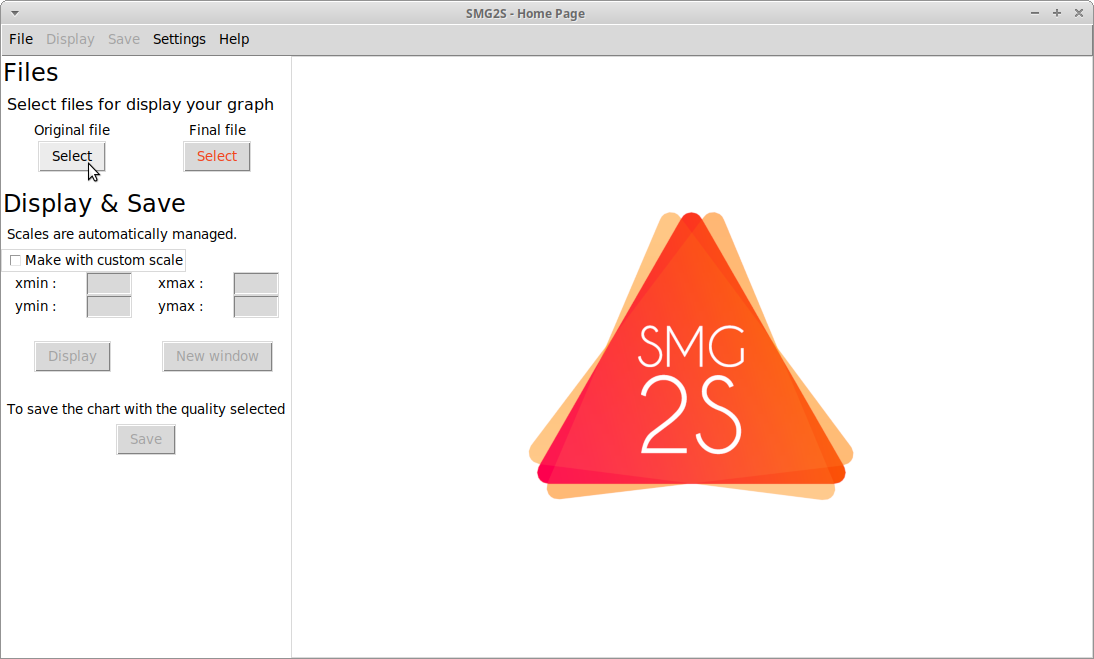
\includegraphics[width=6.2in]{fig/home.png}
	\label{fig:Homescreen}
\end{figure}

The files which store the original spectrum and final eigenvalues can be respectively loaded from local filesystems into the GUI. After that, you can click on "Display" to build and open the graphic on the right side of the window, as shown by Fig. \ref{fig:Home Screen Plot Capture}.

\begin{figure}[htbp]
	\caption{Home Screen Plot Capture}
	\centering
	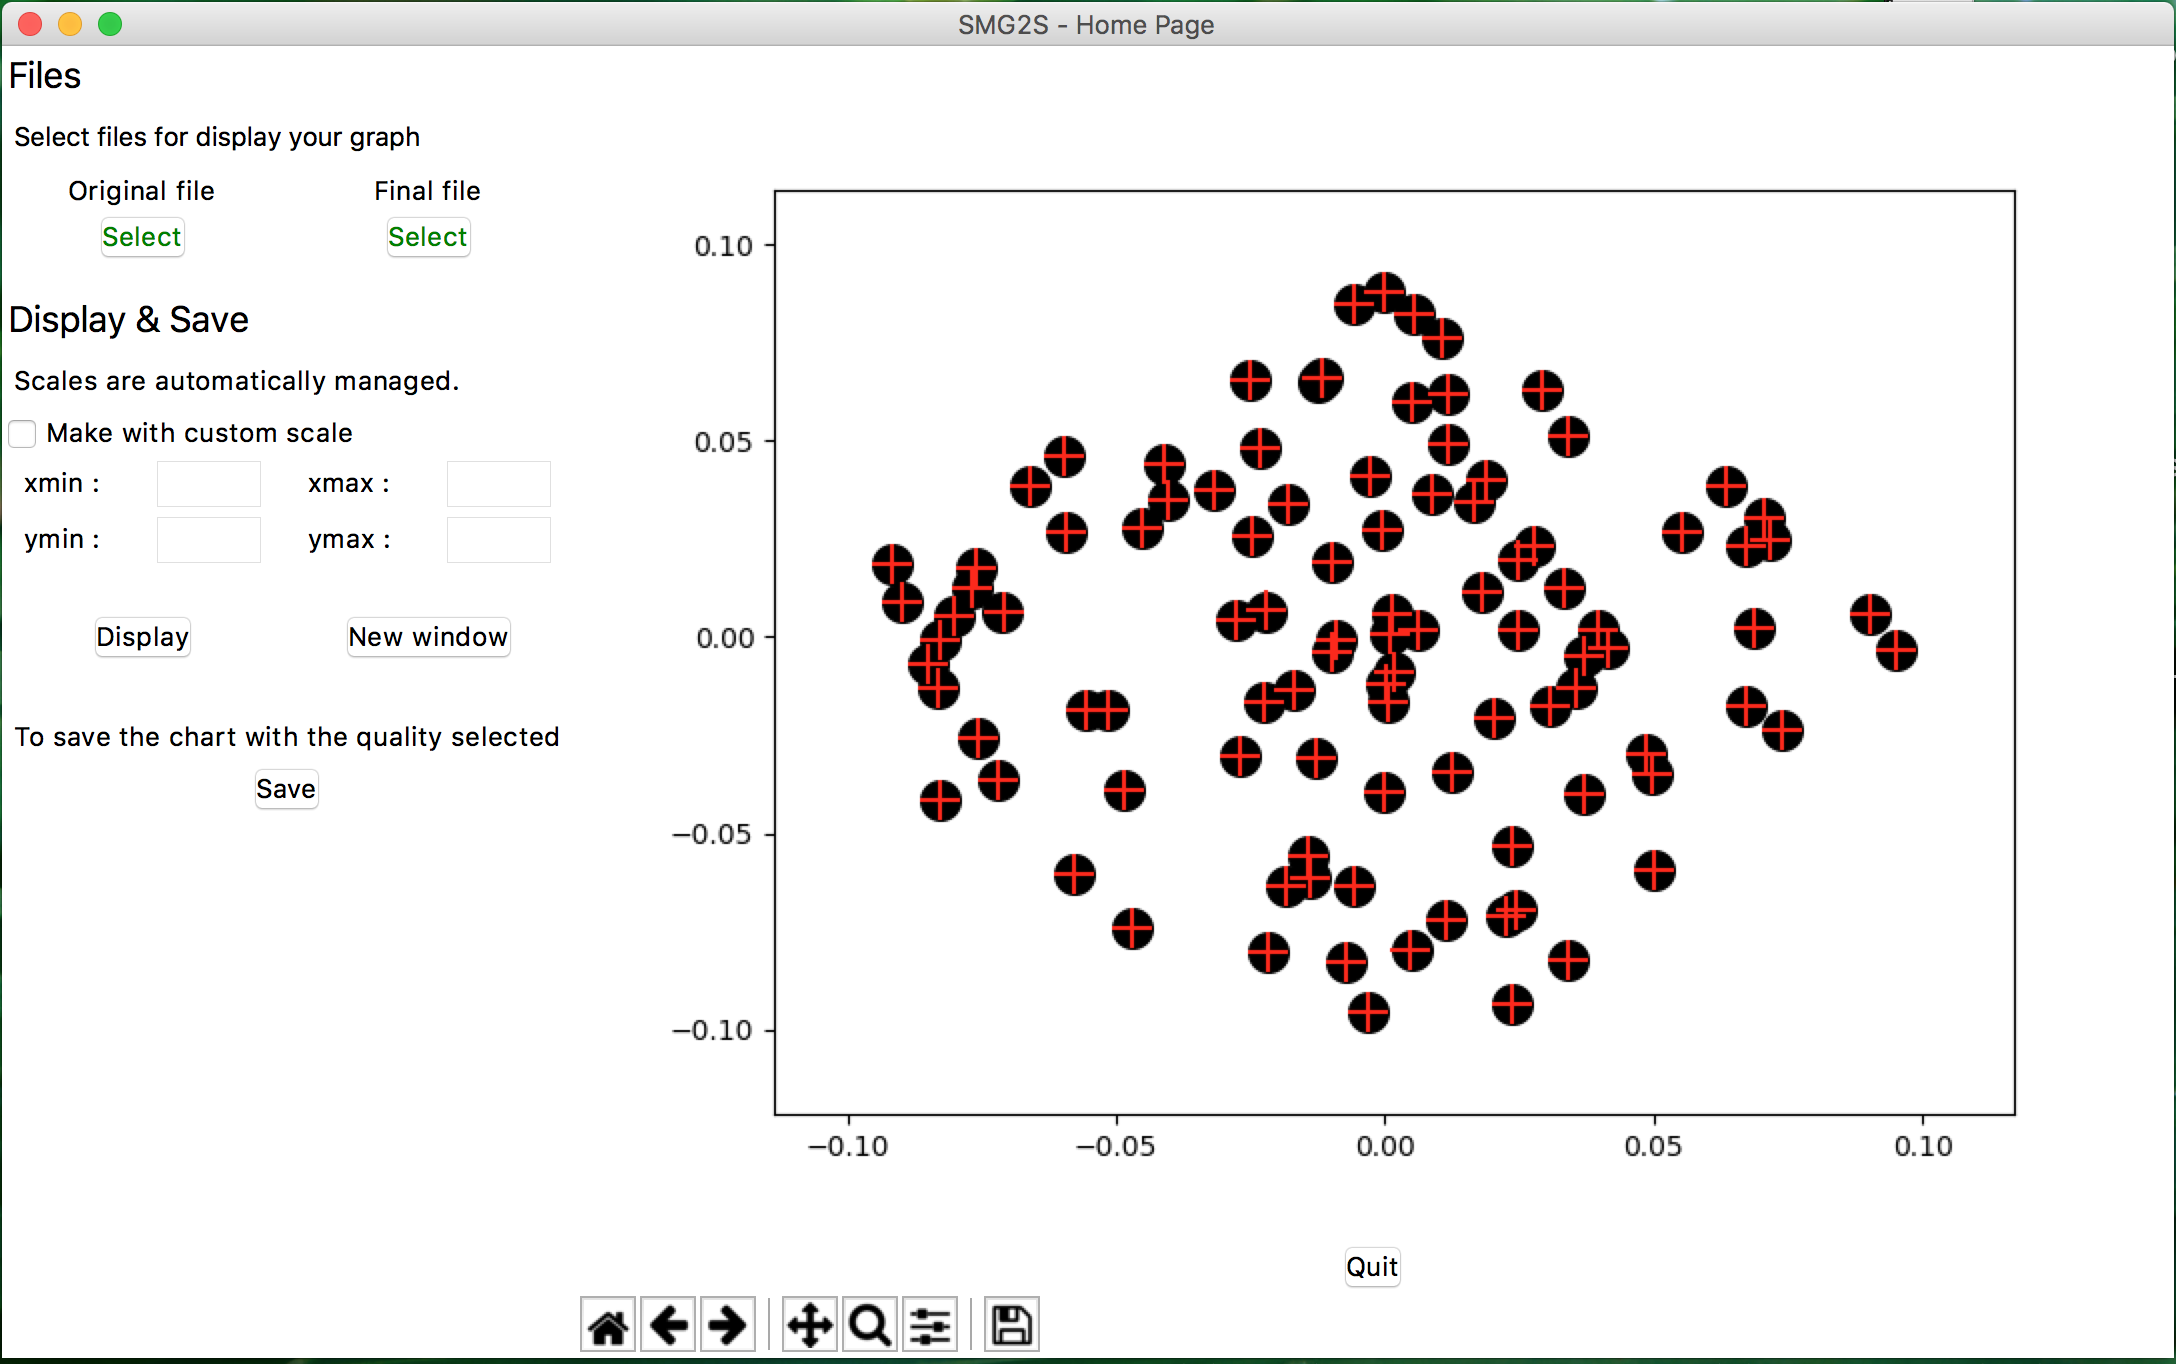
\includegraphics[width=6.2in]{fig/home_screen.png}
	\label{fig:Home Screen Plot Capture}
\end{figure}

This GUI also supports the zoom in/out a small part of figures, which allows the users to see more details of spectral distribution. In addition, the display can also be done with the users' selected scale by inputting the min-max values for the x-axis and y-axis, as shown by Fig. \ref{fig:Home Screen custom}.

\begin{figure}[htbp]
	\caption{Home Screen Custom}
	\centering
	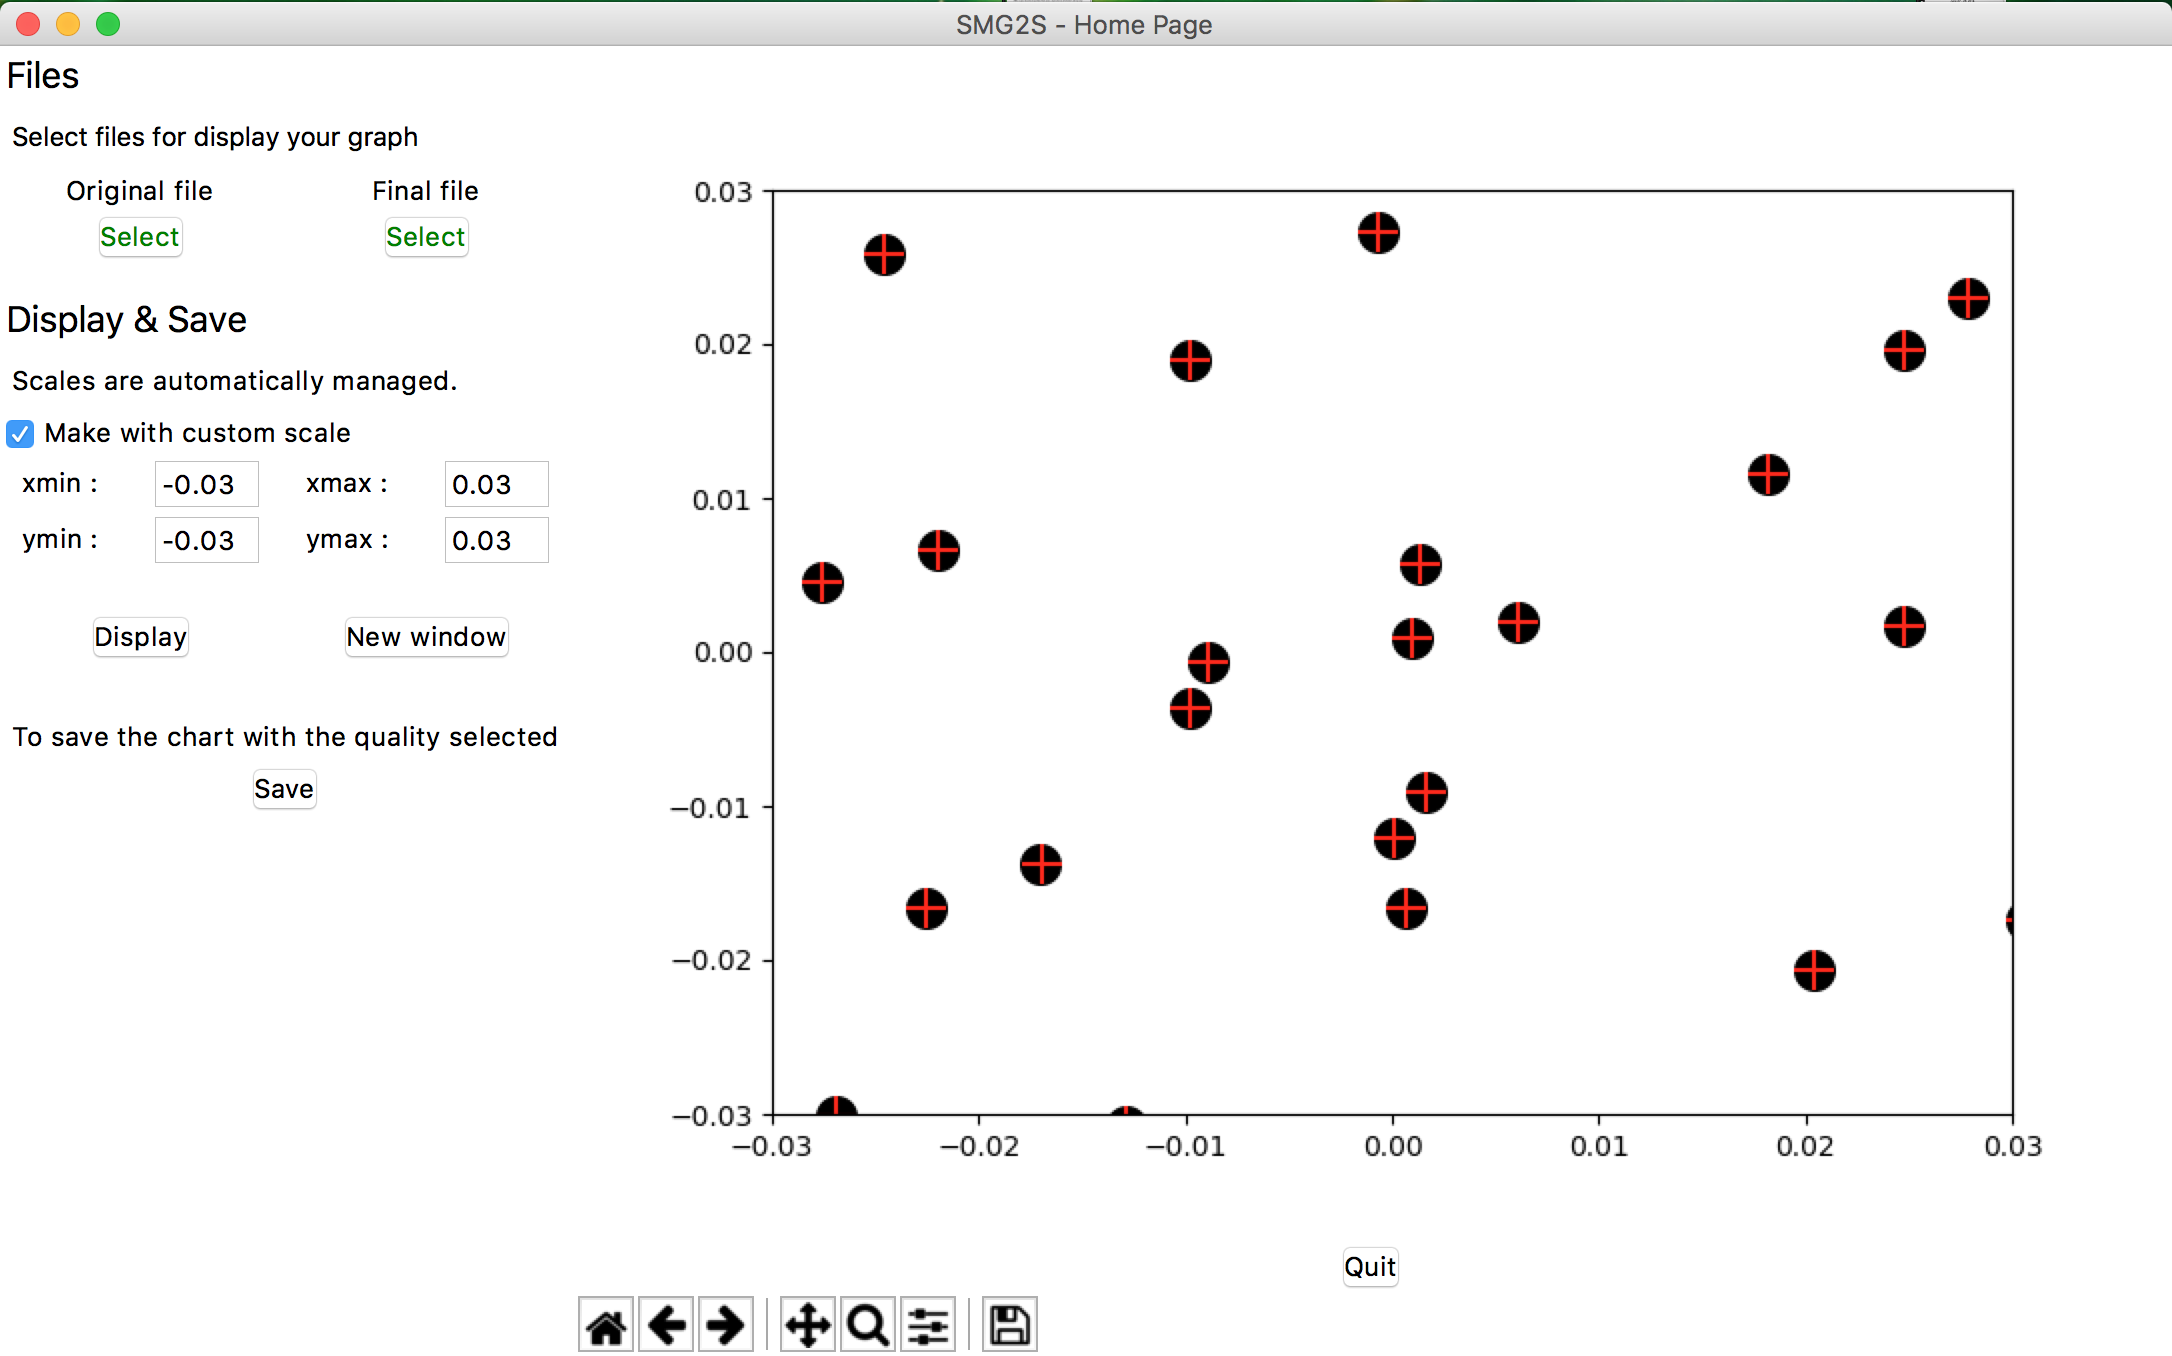
\includegraphics[width=6.2in]{fig/home_screen_custom.png}
	\label{fig:Home Screen custom}
\end{figure}


\section{Krylov Solvers Evaluation using SMG2S}\label{application}

SMG2S is suitable to evaluate different kinds of linear system and eigenvalue solvers. We give an example to demonstrate its workflow by evaluating the Krylov solvers. In this section, we do not mean to propose new points on the Krylov methods, but to show the benefits of SMG2S. A class of Krylov subspace iterative methods is one of the most powerful tools to solve large and sparse linear systems. Their significant advantages such as low memory requirements and a good approximation of solution make them widely be used in applications throughout science and engineering. Convergence analysis of these methods is not only of great theoretical importance, but it can also help to answer practically relevant questions about improving their performance using the preconditioners. The convergence of Krylov solvers depends on the spectral distribution of matrices. And most preconditioners are applied to change the spectral distribution in order to accelerate the convergence. Anyway, the spectrum has a significant impact on the convergence of Krylov methods. We can use SMG2S to generate the test matrices with different spectral distributions and to study their influence on the convergence.

\subsection{SMG2S workflow to evaluate Krylov Solvers}

SMG2S workflow for evaluating the solvers is shown in Fig. \ref{fig:interface}. It generates the matrix in parallel, which means that the different parts of the matrix are already distributed into the computing units of the platform. The interfaces provided to PETSc, Trilinos, and other public or personal parallel solvers, can restore the distributed data into the necessary data structures of different libraries. This feature can significantly reduce the I/O of applications and improve their efficiency to evaluate the numerical methods.

\begin{figure}[t]
	\centering
	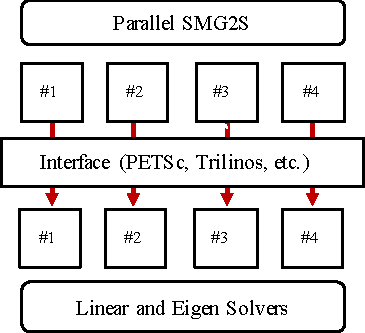
\includegraphics[width=0.64\linewidth]{fig/interface.pdf}
	\caption{SMG2S Workflow and Interface.}
	\label{fig:interface}
\end{figure}


\subsection{Experiments}

We evaluate three different restarted Krylov linear system solvers by SMG2S. The test methods include GMRES, BiCGStab, and TFQMR, with/without the basic parallel preconditioners SOR or Jacobi. In the experiments, matrices with different spectral distributions are generated by SMG2S, including the clustered, closest, conjugate eigenvalues, eigenvalues with dominant values, etc. With the interface implemented between SMG2S and PETSc, we use the parallel Krylov solvers and preconditioners provided by PETSc to do the evaluations.

\begin{figure}[t]
	\caption{Convergence Comparison using a matrix generated by SMG2S.}
	\centering
	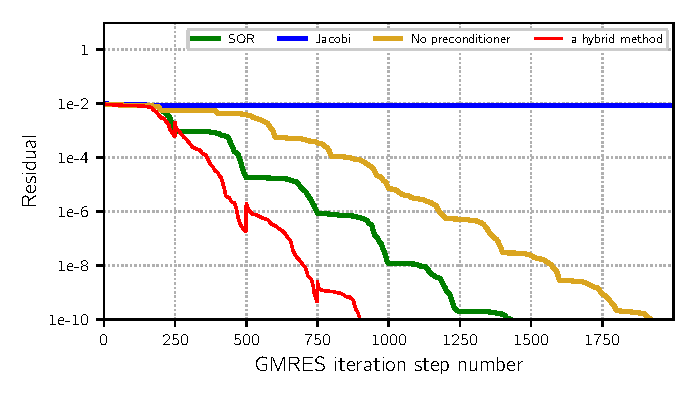
\includegraphics[width=0.99\linewidth]{fig/smg2s_convergence.eps}
		\label{fig:smg2s-convergence}
\end{figure}


\begin{table*}[t]
	\caption{Krylov Solvers Evaluation by SMG2S with matrix row number = \num[round-precision=2,round-mode=figures]{100000}, convergence tolerance = \num[round-precision=2,round-mode=figures]{0.0000000001} (dnc = do not converge in  \num[round-precision=2,round-mode=figures]{80000} iterations, the solvers and preconditioners are provided by PETSc.)}
	\label{krylov}
	\centering
	\footnotesize
	\renewcommand{\arraystretch}{1.5}
	\begin{tabular}{c|c|c|c|c|c|c|c}
		\toprule
		\cellcolor{gray!50}\textbf{Krylov Methods} & 	\cellcolor{gray!50}\textbf{Preconditioner} & 	\cellcolor{gray!50}\textbf{Case 1} & 	\cellcolor{gray!50}\textbf{Case 2} 
		& 	\cellcolor{gray!50}\textbf{Case 3} & 	\cellcolor{gray!50}\textbf{Case 4} & 	\cellcolor{gray!50}\textbf{Case 5} & 	\cellcolor{gray!50}\textbf{Case 6} \\ 
		\midrule
		\multirow{3}{*}{GMRES} & None & 2160 & dnc
		& dnc & dnc &50773 & dnc\\ 
		\cline{2-8}
		& 	\cellcolor{gray!20}Jacobi& 	\cellcolor{gray!20}17 & 	\cellcolor{gray!20}dnc & 	\cellcolor{gray!20}129 & 	\cellcolor{gray!20}dnc &	\cellcolor{gray!20}12056 & 	\cellcolor{gray!20}dnc\\
		\cline{2-8}
		& SOR& 3 &dnc & 4 &dnc & dnc & dnc\\
		\hline
		\multirow{3}{*}{BiCGStab} & 	\cellcolor{gray!20}None & \cellcolor{gray!20}220 & \cellcolor{gray!20}6859
		& \cellcolor{gray!20}dnc&\cellcolor{gray!20}771 &\cellcolor{gray!20}53 &\cellcolor{gray!20}dnc\\ 
		\cline{2-8}
		& Jacobi& 9& 1097 & 66 &214 & 56 &dnc\\
		\cline{2-8}
		& \cellcolor{gray!20}SOR&\cellcolor{gray!20}2 &\cellcolor{gray!20}168 & \cellcolor{gray!20}3 & \cellcolor{gray!20}12 & \cellcolor{gray!20}8& \cellcolor{gray!20}dnc\\
		\hline
		\multirow{3}{*}{TFQMR} & None & 510 & dnc
		& dnc &dnc &dnc& dnc\\ 
		\cline{2-8}
		& \cellcolor{gray!20}Jacobi& \cellcolor{gray!20}18 & \cellcolor{gray!20}dnc & \cellcolor{gray!20}128 & \cellcolor{gray!20}dnc & \cellcolor{gray!20}dnc& \cellcolor{gray!20}dnc\\
		\cline{2-8}
		& SOR& 3&dnc &  5&22 &dnc& dnc\\
		\bottomrule
		
	\end{tabular}
\end{table*}

Fig. \ref{fig:smg2s-convergence} shows the comparsion of conventional GMRES without preconditioning, GMRES preconditioned by Jacobi and SOR, and a hybrid GMRES with Least Squares polynomial, using the matrix generated SMG2S. This figure demonstrates that it is effective to evaluate the convergence of different implementation of GMRES by SMG2S.

Table \ref{krylov} shows iterative steps for convergence of different solvers. We can conclude that different matrices generated by SMG2S with different spectral distributions have divers convergence performance with different solvers and preconditioners. The six cases listed in Table \ref{krylov} are not cover much more different types of spectral distributions, and the tested preconditioners are relatively simple because it is not the primary purpose of this paper. But we can say that SMG2S is a reliable tool which can be used to evaluate the different numerical methods, and in the future, we will make use of it to do more tests with different solvers and novel preconditioners and to analyze their performance with different spectral distributions.

\section{Conclusion and Pespectives}\label{conclusion}

In this chapter, we have presented a scalable matrix generator with the given spectra and its parallel implementation on homogeneous and heterogeneous clusters. This method allows generating large-scale test matrices with customized eigenvalues to evaluate the influence of spectra on the linear and eigenvalue solvers targeting the large-scale platform. We have evaluated the parallel scalability and the accuracy to keep the spectra of matrices generated by this matrix generator. The experiments proved that this method has good scalability and acceptable accuracy to keep the given spectra. One more important benefit of SMG2S is that the matrices are generated in parallel. Thus the data are already allocated to different processes. These distributed data can be used directly for the users to efficiently evaluate the numerical linear methods of the scientific libraries or their personal implementation without concerning the I/O operation, whose time consumption is enormous if the matrix size is large. In the future, in order to augment the bandwidth of the generated matrix, a special data structure and function for the very large factorial operation should be implemented. And the interface to more scientific linear and eigenvalue solver libraries should be provided.


\clearemptydoublepage
